\documentclass[12pt,a4paper]{article}

% Package imports
\usepackage[utf8]{inputenc}
\usepackage[english]{babel} % Changed from spanish to english
\usepackage{geometry}
\usepackage{graphicx}
\usepackage{amsmath}
\usepackage{amssymb}
\usepackage{float}
\usepackage{hyperref}
\usepackage{caption}
\usepackage{subcaption}
\usepackage{booktabs}
\usepackage{multirow}
\usepackage{xcolor}
\usepackage{listings}
\usepackage{fancyhdr}
\usepackage{enumitem}
\usepackage{algorithm}
\usepackage{algpseudocode}

% Page geometry
\geometry{
    left=2.5cm,
    right=2.5cm,
    top=3cm,
    bottom=3cm
}

% Header and footer
\pagestyle{fancy}
\fancyhf{}
\fancyhead[L]{\leftmark}
\fancyhead[R]{\thepage}
\renewcommand{\headrulewidth}{0.4pt}

% Hyperref setup
\hypersetup{
    colorlinks=true,
    linkcolor=blue,
    filecolor=magenta,
    urlcolor=cyan,
    citecolor=green,
}

% Code listing style
\lstset{
    basicstyle=\ttfamily\small,
    breaklines=true,
    frame=single,
    numbers=left,
    numberstyle=\tiny,
    keywordstyle=\color{blue},
    commentstyle=\color{gray},
    stringstyle=\color{red}
}

% Title information
\title{
    \vspace{-2cm}
    \textbf{NIR Spectral Analysis and Dimensionality Reduction for the Classification of Stress Treatments in Plants}\\
    \large Computer Graphics and Scientific Visualization
}
\author{Ricardo Lopera V.}
\date{\today}

\begin{document}

\maketitle

\begin{abstract}
This report presents a comprehensive study on the analysis of near-infrared (NIR) reflectance spectral data for the classification of plants subjected to different stress treatments. The work covers multiple stages: from initial data exploration and scientific visualization, through dimensionality reduction techniques, to the development and evaluation of machine learning models for multiclass classification. Principal Component Analysis (PCA) and t-SNE techniques were implemented to reduce the dimensionality of spectral data comprising over 2,150 wavelengths (350-2500 nm). Subsequently, four classification models were developed and optimized: K-Nearest Neighbors (KNN), Support Vector Machines (SVM), Multilayer Perceptrons (MLP), and Bagging with decision trees. The results demonstrate that NIR spectroscopy techniques combined with machine learning methods can effectively detect different types of stress in plants, with important implications for precision agriculture and non-invasive monitoring of plant health.
\end{abstract}

\tableofcontents
\newpage

\section{Introduction}

\subsection{Context and Motivation}

Plant health and their response to different types of stress (biotic and abiotic) are fundamental to modern agriculture and global food security. Traditional methods for diagnosing plant stress are destructive, slow, and require extensive laboratory analysis. Near-infrared (NIR) reflectance spectroscopy emerges as a non-invasive and rapid alternative that allows assessing the physiological state of plants by analyzing their spectral reflectance patterns.

The NIR spectral range (700-2500 nm) is particularly sensitive to the biochemical composition of plant tissues, including water content, proteins, carbohydrates, and other organic compounds that change in response to stress. However, NIR spectral data present significant challenges: high dimensionality (thousands of wavelengths), collinearity between adjacent variables, and complex non-linear relationships between reflectance and physiological states.

\subsection{Objectives}

The main objectives of this work are:

\begin{enumerate}[label=\arabic*.]
    \item Develop scientific visualization methodologies for high-dimensional spectral data that facilitate the exploration and understanding of patterns in the data.
    \item Apply and compare dimensionality reduction techniques (PCA and t-SNE) to transform complex spectral data into lower-dimensional representations that preserve relevant structure.
    \item Implement and optimize supervised classification models to distinguish between different stress treatments based solely on spectral signatures.
    \item Comparatively evaluate the performance of different model architectures and determine the best hyperparameter configurations through exhaustive search.
    \item Identify the most informative spectral regions for discriminating between treatments through PCA loadings analysis.
\end{enumerate}

\subsection{Document Structure}

This report is organized as follows: Section \ref{sec:data} describes the dataset and experimental treatments; Section \ref{sec:visualization} presents the scientific visualization techniques developed; Section \ref{sec:dimreduction} details the dimensionality reduction methods applied; Section \ref{sec:models} describes the classification models implemented; Section \ref{sec:results} presents the experimental results; and finally, Section \ref{sec:conclusions} discusses the conclusions and future work.

\newpage
\section{Data Description}
\label{sec:data}

\subsection{Dataset}

The dataset used comes from NIR reflectance spectroscopy measurements taken on plants subjected to different stress conditions. The data were collected in the spectral range of 350 to 2500 nm with a spectral resolution of 1 nm, resulting in approximately 2,150 spectral variables per sample.

\subsubsection{Data Structure}

The data were organized into four sheets of an Excel file, each corresponding to different experimental sessions. Each record contains:

\begin{itemize}
    \item \textbf{Plant identifier}: Unique code for each sample
    \item \textbf{Treatment applied}: Category of stress or combination of stresses
    \item \textbf{Reflectance values}: 2,150+ measurements corresponding to each wavelength in the 350-2500 nm range
\end{itemize}

\subsection{Experimental Treatments}

The plants were subjected to the following stress treatments:

\begin{enumerate}
    \item \textbf{Control}: Plants without any stress, maintained in optimal conditions
    \item \textbf{Water Stress (E\_Hidrico)}: Plants subjected to water restriction
    \item \textbf{Fusarium}: Plants inoculated with the pathogenic fungus \textit{Fusarium} sp.
    \item \textbf{Ralstonia}: Plants infected with the bacterium \textit{Ralstonia solanacearum}
    \item \textbf{Fusarium + Water Stress (Fus\_EH)}: Combination of biotic stress (Fusarium) and abiotic stress (drought)
    \item \textbf{Ralstonia + Water Stress (Ral\_EH)}: Combination of biotic stress (Ralstonia) and abiotic stress (drought)
    \item \textbf{Fusarium + Water Stress + Ralstonia (Fus\_EH\_Ral)}: Triple stress combining both pathogens and drought
\end{enumerate}

\subsection{Data Preprocessing}

Data from the four experimental sheets were concatenated into a single DataFrame for analysis. Data integrity and the absence of missing values were verified. Since the spectral measurements were already normalized as reflectance values (0-1), no additional normalization was required at this initial stage.

For subsequent analyses, the data were divided into:
\begin{itemize}
    \item \textbf{Feature matrix (X)}: All spectral columns (wavelengths)
    \item \textbf{Target vector (y)}: Treatment labels
\end{itemize}

The training-test split was performed using class stratification with 90\% of the data for training and 10\% for evaluation, ensuring proportional representation of each treatment in both sets.

\newpage
\section{Scientific Visualization of Spectral Data}
\label{sec:visualization}

\subsection{Motivation and Challenges}

Effective visualization of high-dimensional spectral data presents unique challenges. With over 2,000 wavelengths per sample and multiple treatments to compare, it is essential to develop graphical representations that are:

\begin{itemize}
    \item \textbf{Informative}: Revealing patterns, trends, and differences between treatments
    \item \textbf{Interpretable}: Allowing identification of relevant spectral regions
    \item \textbf{Publishable}: Of sufficient quality for academic publications
    \item \textbf{Consistent}: With uniform and reusable styles
\end{itemize}

\subsection{Development of Visualization Templates}

A modular system of visualization functions with an academic style was developed, inspired by high-impact scientific publications. The main features include:

\subsubsection{Custom Visual Style}

A base style was configured using matplotlib and seaborn with the following specifications:

\begin{itemize}
    \item \textbf{Typography}: LaTeX-style serif fonts (Computer Modern Roman) for consistency with academic documents
    \item \textbf{Color palette}: Vivid and distinct colors for maximum distinguishability between groups
    \item \textbf{Grids}: Visible grids with controlled transparency to facilitate value reading
    \item \textbf{Axes and frames}: Defined borders with removal of top and right spines for visual cleanliness
\end{itemize}

\subsubsection{Visualization of Spectral Curves}

The main function developed allows plotting the average spectral curves for each treatment in the full NIR range (350-2500 nm). Figure \ref{fig:spectral_curves} shows an example of this visualization.

\begin{figure}[H]
    \centering
    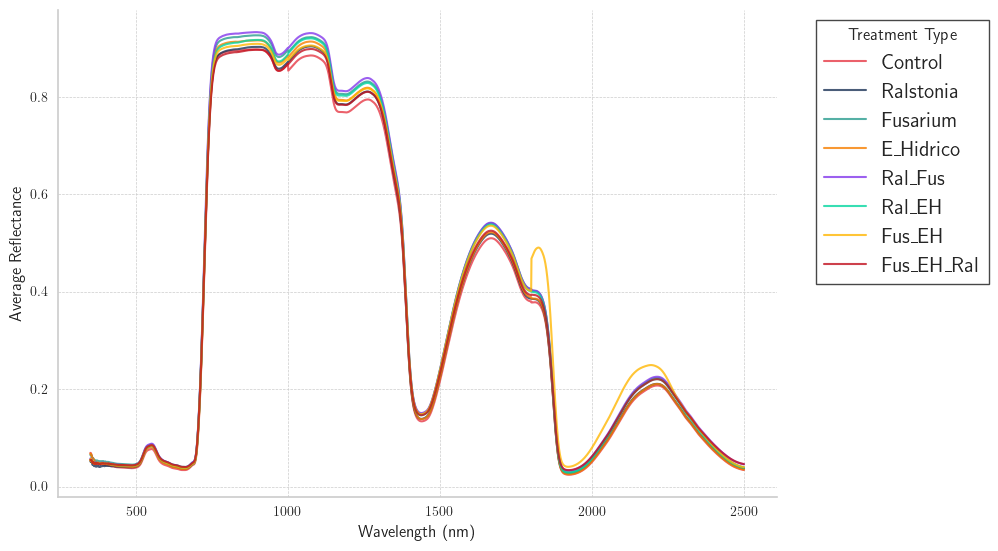
\includegraphics[width=0.9\textwidth]{Plots/Average_NIR_Spectrar_reponce_by_treatment}
    \caption{Average NIR spectral response (350-2500 nm) for each treatment. }
    \label{fig:spectral_curves}
\end{figure}

Each line represents the average of all plants subjected to a specific treatment. Differences between curves indicate changes in reflectance associated with different types of stress.

\subsection{Visualization with Zoom (Inset Plots)}

To examine specific spectral regions of interest, zoom functionality was implemented using inset plots. This technique allows for:

\begin{itemize}
    \item Visualizing the full spectrum in the main graph
    \item Showing a magnified region in an inserted box
    \item Visually connecting both regions with indicator lines
\end{itemize}

Figure \ref{fig:spectral_zoom} illustrates this technique applied to the 700-1370 nm NIR region, where notable differences between treatments are observed.

\begin{figure}[H]
    \centering
    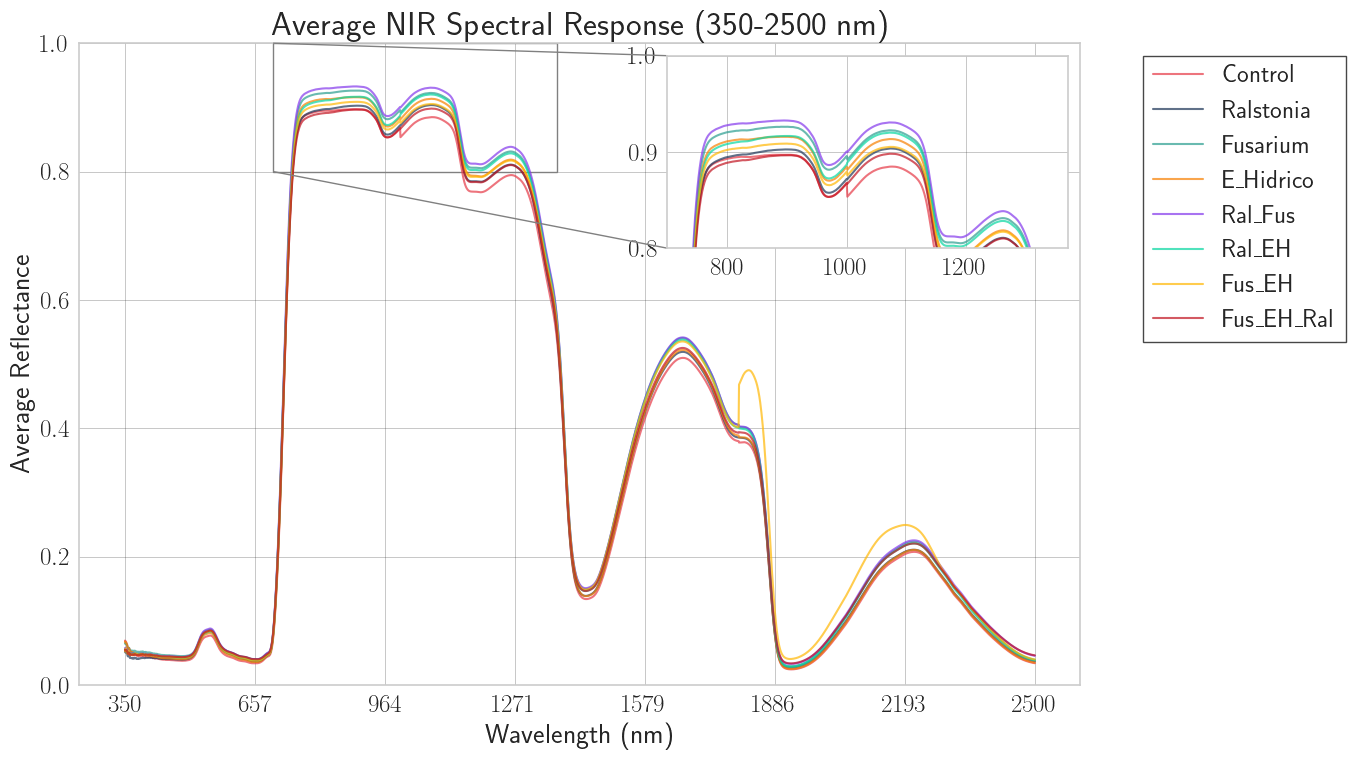
\includegraphics[width=0.9\textwidth]{Plots/ZOOM.png}
    \caption{Spectral curves with zoom in the 700-1370 nm region. }
    \label{fig:spectral_zoom}
\end{figure}

The inserted box shows an enlargement of the region of interest, where differences between treatments are more pronounced. This region corresponds to the near-NIR, sensitive to water content and cellular structure.

\subsection{Implemented Plot Types}

A versatile function was developed that supports multiple types of visualization:

\begin{enumerate}
    \item \textbf{Line plot (line)}: To visualize continuous trends in the spectrum
    \item \textbf{Scatter plot (scatter)}: To emphasize individual data points
    \item \textbf{Area plot (area)}: To visualize cumulative magnitudes
    \item \textbf{Lollipop plot (lollipop)}: For discrete comparisons between wavelengths
    \item \textbf{Step plot (step)}: To visualize discrete changes in reflectance
    \item \textbf{Bar plot (bar)}: For direct comparisons between treatments at specific wavelengths
\end{enumerate}

Each plot type is appropriate for different analytical purposes. The flexibility of the function allows selecting the most suitable type according to the message to be communicated.

\subsection{Customization Parameters}

The developed academic visualization function accepts 15+ configurable parameters:

\begin{itemize}
    \item \textbf{Style and palette}: Full control over color schemes and seaborn styles
    \item \textbf{Dimensions}: Configurable figure size for different publication formats
    \item \textbf{Typography}: Independent font sizes for title, labels, and ticks
    \item \textbf{Annotations}: System for adding annotations with arrows and text boxes
    \item \textbf{Transparency}: Alpha control for overlays and shaded areas
    \item \textbf{Markers}: Customization of marker sizes and styles
\end{itemize}

This modularity allows for the generation of consistent, high-quality visualizations with minimal programming effort.

\newpage
\section{Dimensionality Reduction}
\label{sec:dimreduction}

\subsection{Need for Dimensionality Reduction}

NIR spectral data have two characteristics that complicate their direct analysis:

\begin{enumerate}
    \item \textbf{High dimensionality}: With over 2,150 variables (wavelengths), the feature space is extremely large, resulting in the "curse of dimensionality" for many machine learning algorithms.
    \item \textbf{Collinearity}: Adjacent wavelengths are highly correlated, introducing redundancy in the information.
\end{enumerate}

Dimensionality reduction addresses these problems by transforming the data into a lower-dimensional space that retains most of the relevant information, facilitating visualization, exploratory analysis, and improving the performance of classification models.

\subsection{Principal Component Analysis (PCA)}

\subsubsection{Theoretical Foundations}

PCA is a linear dimensionality reduction technique that transforms the original variables into a new set of uncorrelated variables called principal components. Mathematically, PCA finds the directions of maximum variance in the high-dimensional space through eigenvalue decomposition of the covariance matrix:

\begin{equation}
\Sigma = \frac{1}{n-1}X^T X
\end{equation}

where $X$ is the centered data matrix and $\Sigma$ is the covariance matrix. The principal components are the eigenvectors corresponding to the largest eigenvalues of $\Sigma$.

\subsubsection{Implementation of 2D PCA}

PCA was applied with 2 principal components to the spectral data. The results show:

\begin{itemize}
    \item \textbf{PC1}: Captures 61.88\% of the total variance
    \item \textbf{PC2}: Captures 23.21\% of the total variance
    \item \textbf{Total explained variance}: 85.09\%
\end{itemize}

Figure \ref{fig:pca2d} shows the projection of all samples onto the two-dimensional space defined by the first two principal components.

\begin{figure}[H]
    \centering
    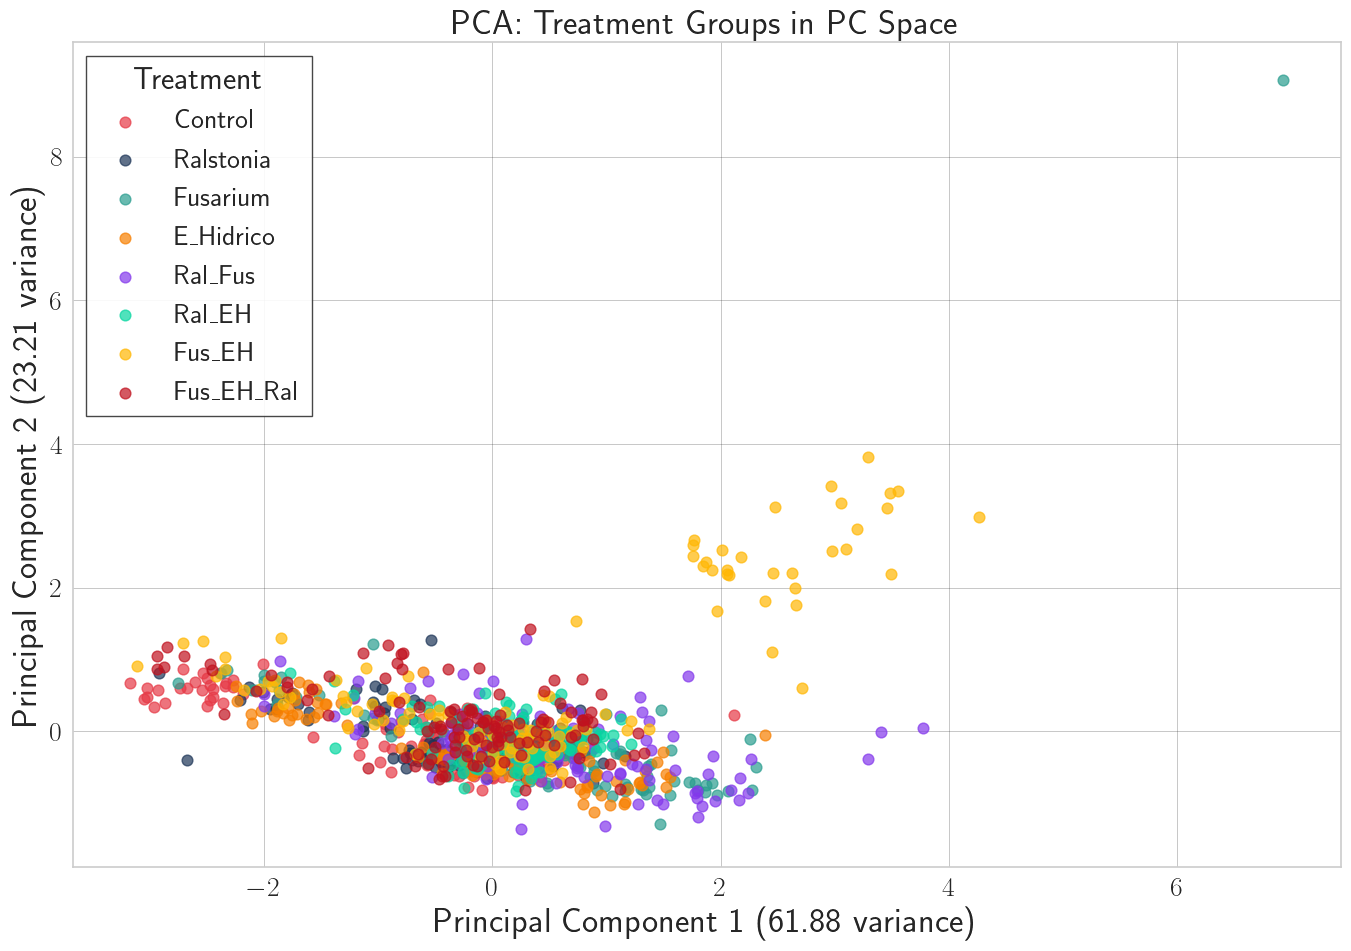
\includegraphics[width=0.9\textwidth]{Plots/2D_PCA.png}
    \caption{2D PCA projection of the spectral data. }
    \label{fig:pca2d}
\end{figure}

Each point represents an individual plant, colored according to its treatment. PC1 (61.88\% variance) primarily separates the control from the stress treatments. PC2 (23.21\% variance) distinguishes between different types of stress. An extreme outlier in the Fusarium treatment is observed (top right corner).

\subsubsection{Loadings Analysis}

PCA loadings reveal which wavelengths contribute most to each principal component. The loadings are the coefficients that relate the original variables to the principal components:

\begin{equation}
PC_i = \sum_{j=1}^{p} w_{ij} \cdot X_j
\end{equation}

where $w_{ij}$ is the loading of variable $j$ on component $i$.

Figure \ref{fig:pca_loadings} visualizes the loadings of PC1 and PC2 across the full spectrum.

\begin{figure}[H]
    \centering
    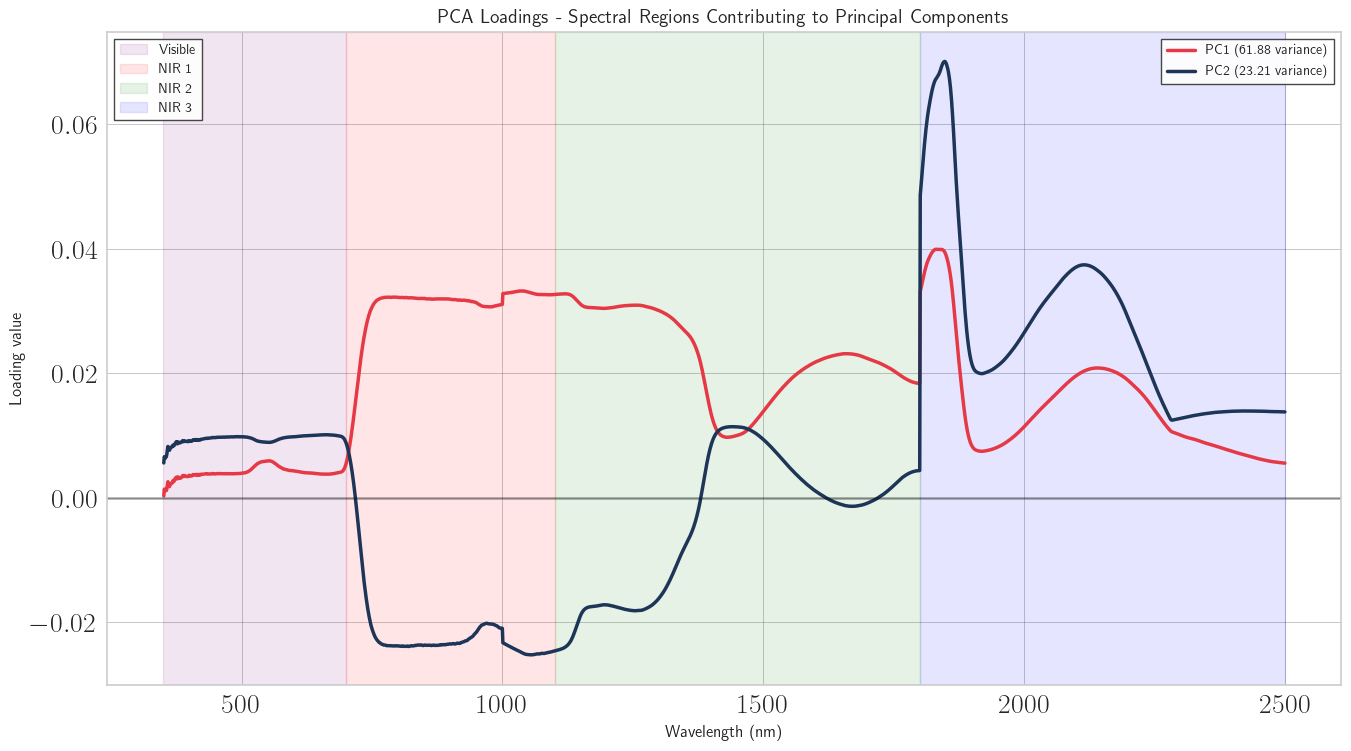
\includegraphics[width=0.9\textwidth]{Plots/2D_PCA_As_WaveLenghts.png}
    \caption{PCA loadings as a function of wavelength. }
    \label{fig:pca_loadings}
\end{figure}

The shaded regions indicate different spectral ranges: visible (350-700 nm), NIR1 (700-1100 nm), NIR2 (1100-1800 nm), and NIR3 (1800-2500 nm). Peaks and valleys in the loadings indicate the most important wavelengths for discriminating between treatments. PC1 shows significant loadings across the entire spectrum, while PC2 shows more localized variations.

\subsubsection{3D PCA}

To capture more variability, the analysis was extended to 3 principal components:

\begin{itemize}
    \item \textbf{PC1}: 61.88\% variance
    \item \textbf{PC2}: 23.21\% variance
    \item \textbf{PC3}: 9.28\% variance
    \item \textbf{Total explained variance}: 94.38\%
\end{itemize}

Figure \ref{fig:pca3d} shows the three-dimensional visualization with emphasis on the Fusarium outlier.

\begin{figure}[H]
    \centering
    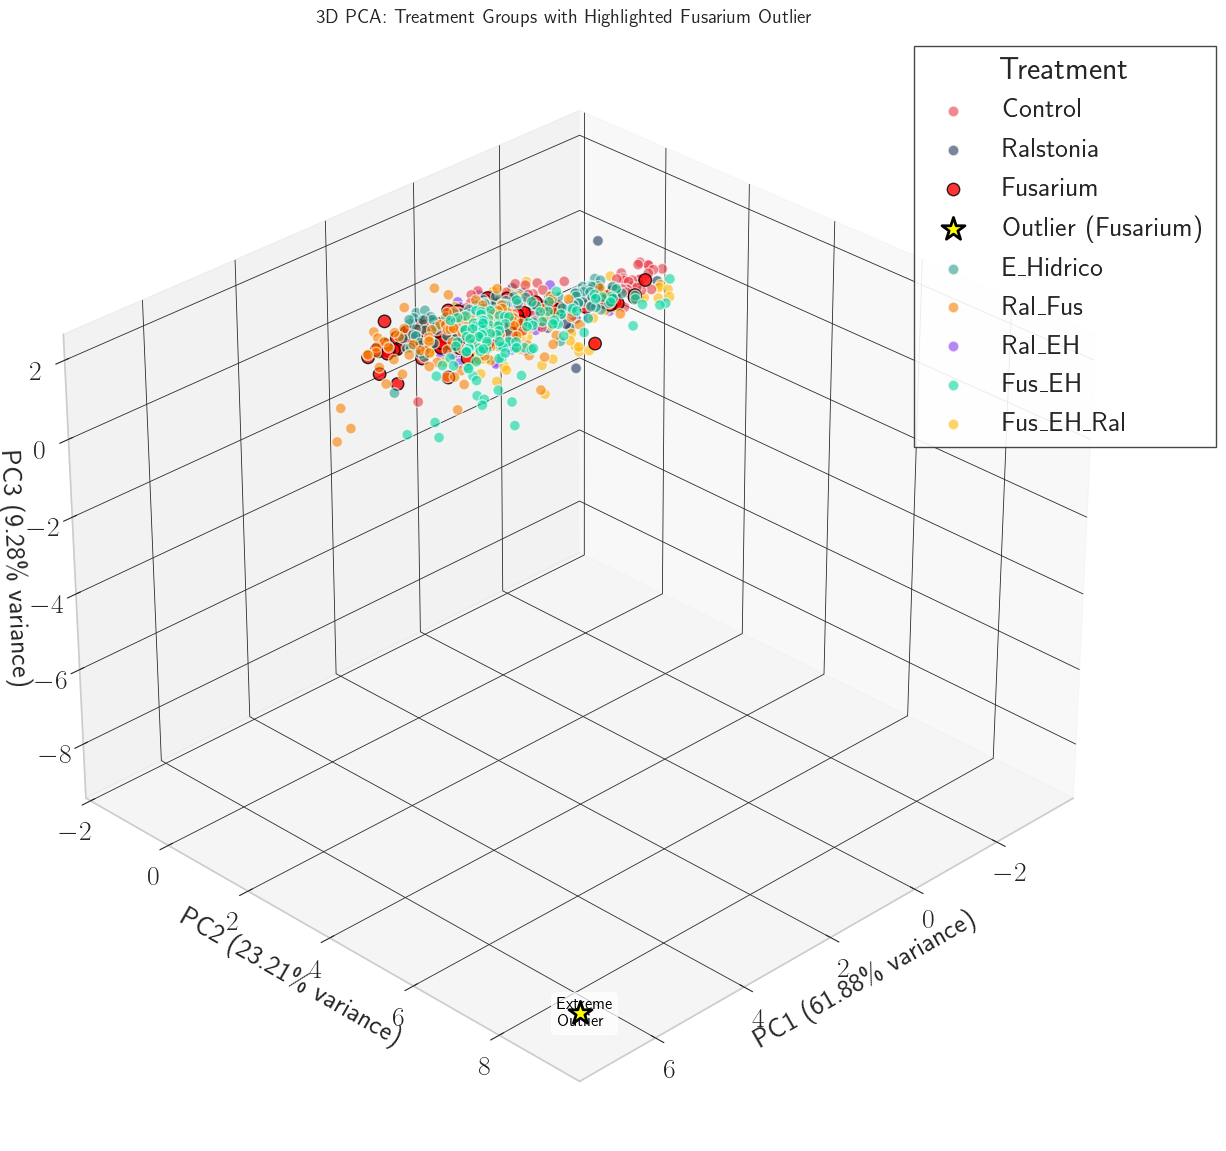
\includegraphics[width=0.9\textwidth]{Plots/3D_PCA.png}
    \caption{3D PCA projection with the Fusarium outlier highlighted with a yellow star. }
    \label{fig:pca3d}
\end{figure}

The third dimension (PC3, 9.28\% variance) provides additional separation between groups. The extreme outlier indicates a unique spectral signature that could correspond to an anomalous physiological response or a measurement error. The Fusarium points (red) stand out from the other treatments.

\subsubsection{Biological Interpretation of PCA}

The PCA analysis reveals two important findings:

\begin{enumerate}
    \item \textbf{Extreme outlier in Fusarium}: A plant treated with Fusarium exhibits a unique spectral signature, located far from all other points in the PCA space. This suggests:
    \begin{itemize}
        \item Possible instrumental measurement error
        \item Exceptional physiological response to the pathogen
        \item Advanced stage of infection not representative of the group
    \end{itemize}
    
    \item \textbf{Separation of combined stress}: Plants subjected to triple stress (Fus\_EH\_Ral) show distinctive spectral signatures, locating in intermediate regions of the PCA space, which indicates that the combined stress produces spectral effects that are combinations of the individual stresses.
\end{enumerate}

\subsection{t-Distributed Stochastic Neighbor Embedding (t-SNE)}

\subsubsection{Foundations of t-SNE}

Unlike PCA, which is a linear method, t-SNE is a non-linear technique designed specifically for visualization. t-SNE operates in two stages:

\begin{enumerate}
    \item \textbf{Similarities in high dimension}: Calculates conditional probabilities that represent similarities between points in the original space:
    \begin{equation}
    p_{j|i} = \frac{\exp(-||x_i - x_j||^2 / 2\sigma_i^2)}{\sum_{k \neq i} \exp(-||x_i - x_k||^2 / 2\sigma_i^2)}
    \end{equation}
    
    \item \textbf{Similarities in low dimension}: Defines similarities in the reduced space using a Student's t-distribution:
    \begin{equation}
    q_{ij} = \frac{(1 + ||y_i - y_j||^2)^{-1}}{\sum_{k \neq l} (1 + ||y_k - y_l||^2)^{-1}}
    \end{equation}
\end{enumerate}

The algorithm minimizes the Kullback-Leibler divergence between these two distributions:

\begin{equation}
KL(P||Q) = \sum_{i \neq j} p_{ij} \log \frac{p_{ij}}{q_{ij}}
\end{equation}

\subsubsection{2D t-SNE}

t-SNE was applied with perplexity=30 (a hyperparameter that controls the balance between preserving local and global structure). Figure \ref{fig:tsne2d} shows the results.

\begin{figure}[H]
    \centering
    \includegraphics[width=0.9\textwidth]{Plots/2D_tSNE.png}
    \caption{2D t-SNE visualization of the treatments. }
    \label{fig:tsne2d}
\end{figure}

t-SNE produces more compact and better-separated clusters than PCA, especially for the individual stress treatments. The control forms a well-defined cluster, while the combined stresses show greater dispersion. The final KL divergence was 0.98, indicating successful convergence.

\subsubsection{3D t-SNE}

The extension to three dimensions allows for even more local structure preservation. Figure \ref{fig:tsne3d} presents the three-dimensional visualization.

\begin{figure}[H]
    \centering
    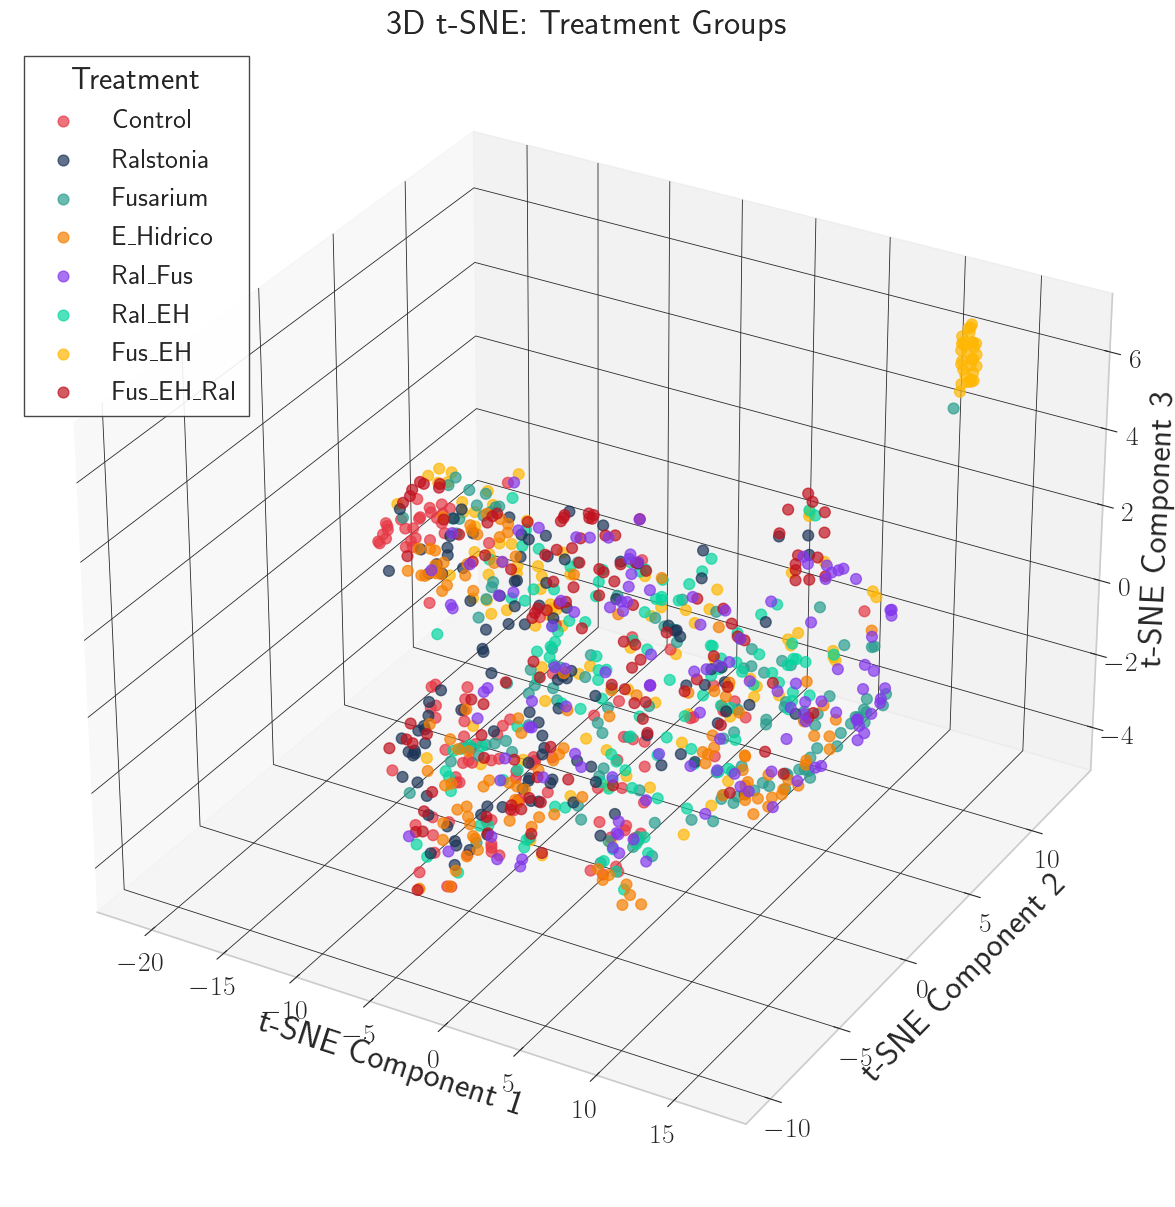
\includegraphics[width=0.9\textwidth]{Plots/3D_SNE.png}
    \caption{3D t-SNE visualization. }
    \label{fig:tsne3d}
\end{figure}

The third dimension provides additional separation between groups, particularly for distinguishing between the different types of combined stress. The clusters are more defined than in 2D, with less overlap between treatments.

\subsection{Quantitative Evaluation: Trustworthiness}

To objectively evaluate how well each method preserves the local neighborhood structure, the trustworthiness score was calculated. This metric assesses whether points that are neighbors in the low-dimensional space were also neighbors in the original space:

\begin{equation}
T(k) = 1 - \frac{2}{nk(2n-3k-1)} \sum_{i=1}^{n} \sum_{j \in U_k(i)} (r(i,j) - k)
\end{equation}

where $U_k(i)$ are the $k$ nearest neighbors of $i$ in the reduced space that were not among its $k$ neighbors in the original space, and $r(i,j)$ is the rank of $j$ in the neighbor list of $i$ in the original space.

The results (Table \ref{tab:trustworthiness}) show that t-SNE surpasses PCA in preserving local structure:

\begin{table}[H]
\centering
\caption{Trustworthiness Scores for different dimensionality reduction methods (k=30 neighbors)}
\label{tab:trustworthiness}
\begin{tabular}{lc}
\toprule
\textbf{Method} & \textbf{Trustworthiness Score} \\
\midrule
t-SNE 3D & 0.9870 \\
t-SNE 2D & 0.9795 \\
PCA 3D & 0.9779 \\
PCA 2D & 0.9747 \\
\bottomrule
\end{tabular}
\end{table}

\subsection{PCA vs t-SNE Comparison}

\begin{table}[H]
\centering
\caption{Feature comparison between PCA and t-SNE}
\label{tab:pca_vs_tsne}
\begin{tabular}{p{4cm}p{5cm}p{5cm}}
\toprule
\textbf{Feature} & \textbf{PCA} & \textbf{t-SNE} \\
\midrule
Transformation type & Linear & Non-linear \\
Objective & Maximize variance & Preserve local neighborhoods \\
Interpretability & High (loadings) & Low \\
Speed & Fast & Slow \\
Determinism & Deterministic & Stochastic \\
Cluster separation & Moderate & Excellent \\
Main use & Preprocessing, feature extraction & Visualization \\
Trustworthiness & 0.9747-0.9779 & 0.9795-0.9870 \\
\bottomrule
\end{tabular}
\end{table}

\textbf{Conclusion}: t-SNE is superior for visualization and cluster exploration, while PCA is more suitable as a preprocessing step for classification models due to its interpretability and computational efficiency.

\newpage
\section{Classification Models (DataFrame without FusEH in sheet 0)}
\label{sec:models}

\subsection{Modeling Strategy}

To evaluate the ability of different machine learning algorithms to classify plants based on their spectral signatures, four distinct approaches were implemented:

\begin{enumerate}
    \item K-Nearest Neighbors (KNN) - Instance-based method
    \item Support Vector Machines (SVM) - Maximum-margin method
    \item Multilayer Perceptron (MLP) - Deep neural network
    \item Bagging with Decision Trees - Ensemble method
\end{enumerate}

All models use PCA as a preprocessing step to reduce dimensionality and improve computational efficiency. Exhaustive hyperparameter search was implemented using GridSearchCV or RandomizedSearchCV with 5-fold cross-validation.

\subsection{Data Splitting}

The data was stratified and split:
\begin{itemize}
    \item \textbf{Training set}: 90\% of the data
    \item \textbf{Test set}: 10\% of the data
    \item \textbf{Stratification}: Proportional by class to maintain treatment distribution
\end{itemize}

\subsection{K-Nearest Neighbors (KNN)}

\subsubsection{Algorithm Foundation}

KNN is a non-parametric classification algorithm that assigns a class to a point based on the classes of its $k$ nearest neighbors in the feature space. The prediction is made by majority vote:

\begin{equation}
\hat{y} = \arg\max_{c} \sum_{i \in N_k(x)} \mathbb{1}(y_i = c)
\end{equation}

where $N_k(x)$ are the $k$ nearest neighbors of $x$.

\subsubsection{Hyperparameter Search Space}

An exhaustive search was implemented over the following space:

\begin{itemize}
    \item \textbf{pca\_\_n\_components}: [3, 5, 10, 20, 30] - Number of principal components
    \item \textbf{knn\_\_n\_neighbors}: [1, 2, 3, 4, 5, 7, 9, 11, 13, 15] - Number of neighbors
    \item \textbf{knn\_\_weights}: ['uniform', 'distance'] - Weighting scheme
    \item \textbf{knn\_\_metric}: ['euclidean', 'manhattan', 'minkowski', 'chebyshev'] - Distance metric
    \item \textbf{knn\_\_p}: [1, 2, 3] - p-parameter for Minkowski distance
    \item \textbf{knn\_\_algorithm}: ['auto', 'ball\_tree', 'kd\_tree', 'brute'] - Search algorithm
    \item \textbf{knn\_\_leaf\_size}: [10, 30, 50, 100] - Leaf size for trees
\end{itemize}

\subsubsection{Processing Pipeline}

The KNN pipeline consists of:

\begin{enumerate}
    \item \textbf{PCA}: Dimensionality reduction
    \item \textbf{KNN}: K-nearest neighbors classifier
\end{enumerate}

\subsubsection{KNN Results}

The best hyperparameters found and the performance on the test set are presented in the following figures.

\begin{figure}[H]
    \centering
    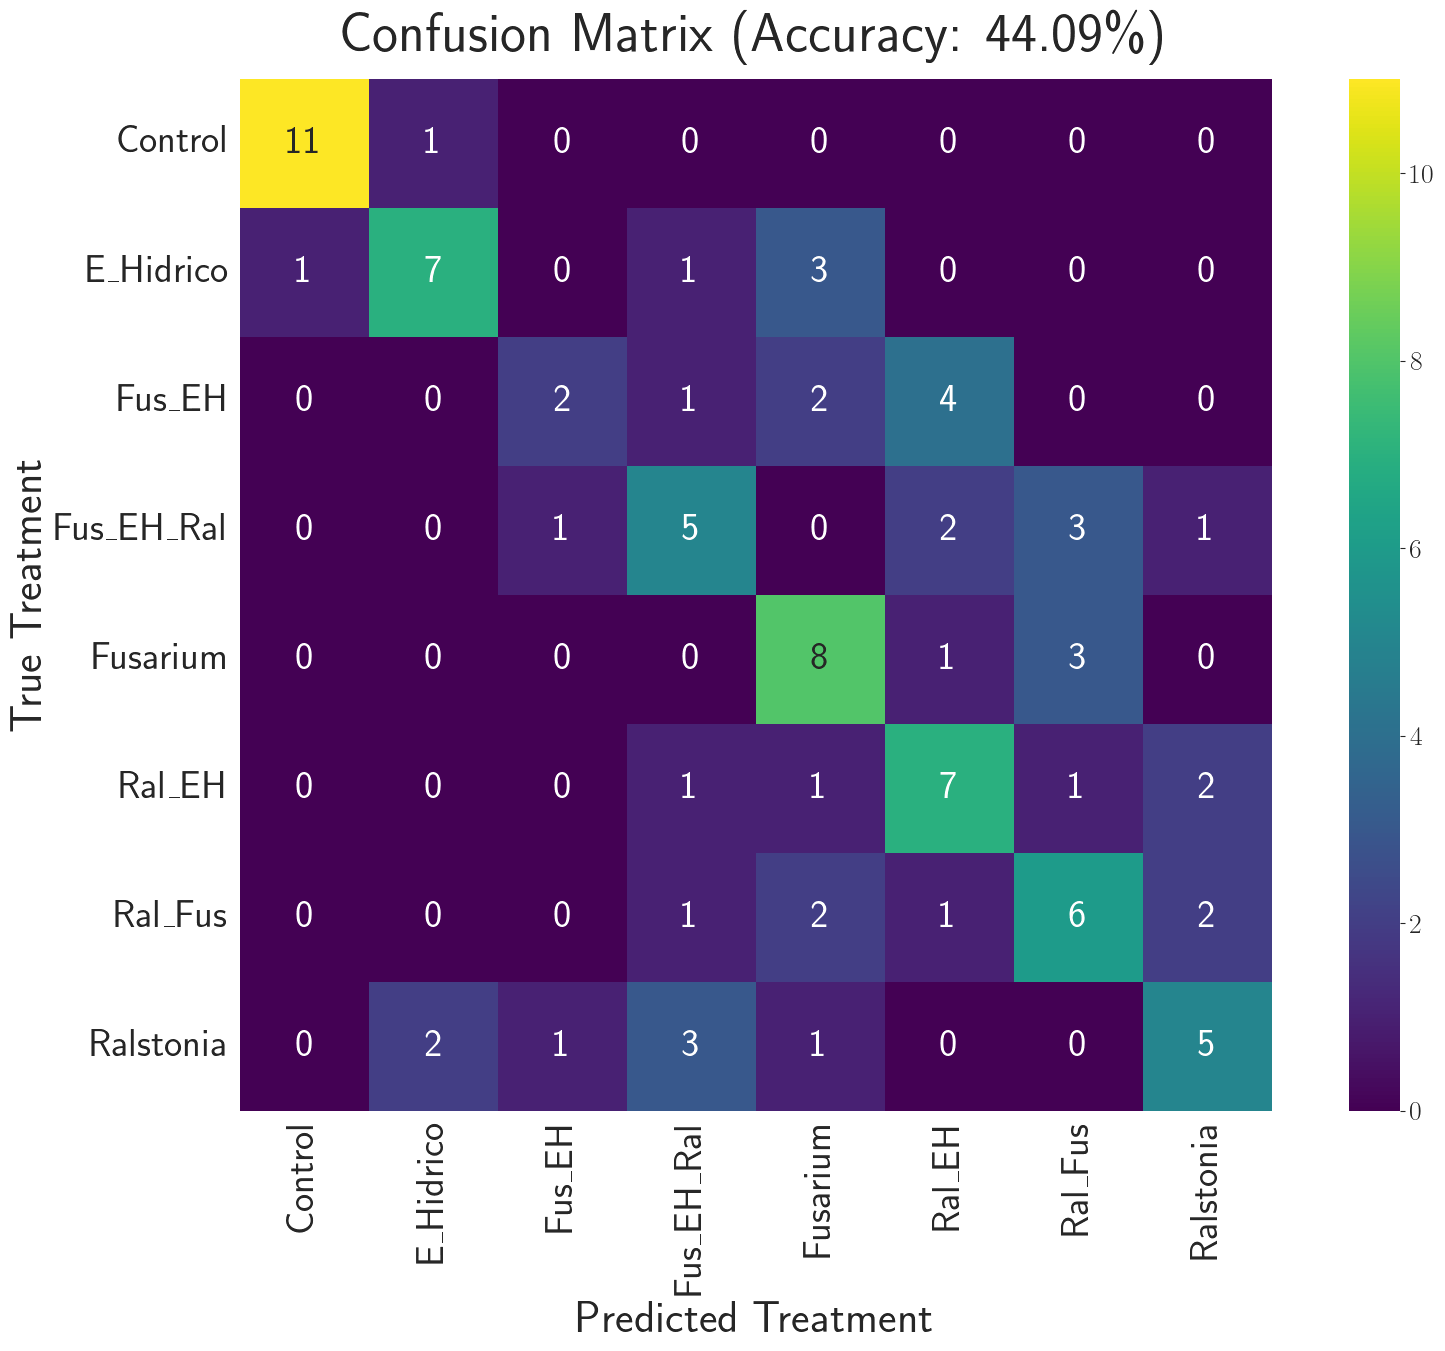
\includegraphics[width=0.8\textwidth]{Plots/KNN_Confussion_Matrix.png}
    \caption{Confusion matrix of the optimized KNN model. }
    \label{fig:knn_confusion}
\end{figure}

The main diagonal shows correct classifications, while off-diagonal elements indicate classification errors. The model shows high accuracy in distinguishing the control and individual stresses, with more confusion between combined stresses.

\begin{figure}[H]
    \centering
    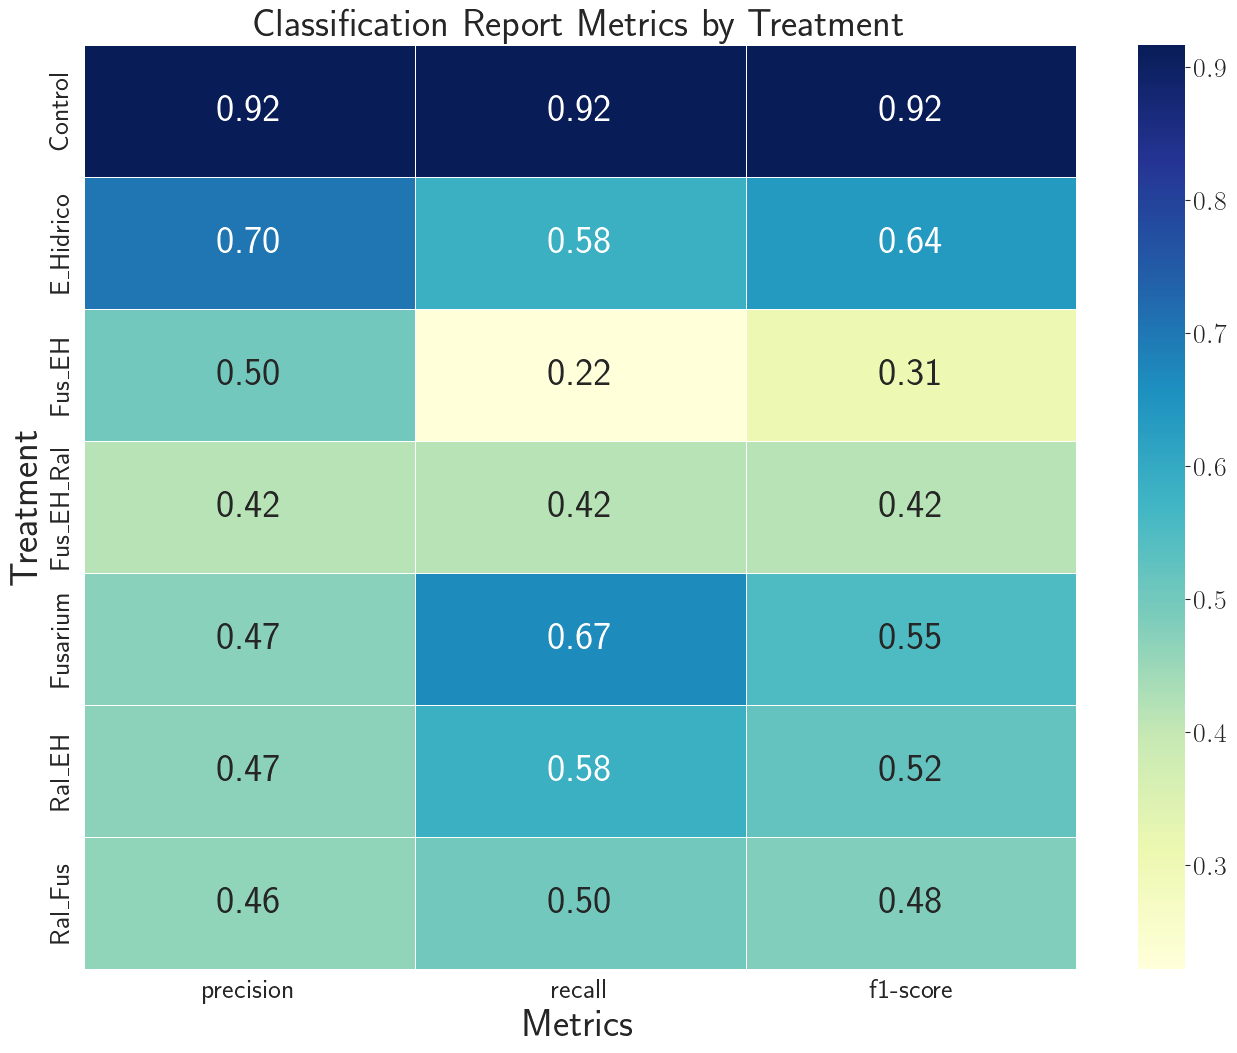
\includegraphics[width=0.8\textwidth]{Plots/KNN_Metrics_Report.png}
    \caption{Performance metrics per class for KNN. }
    \label{fig:knn_report}
\end{figure}

The heatmap shows precision, recall, and F1-score for each treatment. Darker colors indicate better performance. It is observed that the control and single stresses have F1-scores above 0.90, while combined stresses show greater variability.

\subsection{Support Vector Machines (SVM)}

\subsubsection{Algorithm Foundation}

SVM seeks the optimal hyperplane that maximizes the margin between classes. For non-linear problems, it uses the kernel trick to map data to a higher-dimensional space:

\begin{equation}
f(x) = \text{sign}\left(\sum_{i=1}^{n} \alpha_i y_i K(x_i, x) + b\right)
\end{equation}

where $K(x_i, x)$ is the kernel function and $\alpha_i$ are the Lagrange multipliers.

\subsubsection{Hyperparameter Search Space}

\begin{itemize}
    \item \textbf{pca\_\_n\_components}: [5, 10, 15, 20, 30, 40]
    \item \textbf{svm\_\_C}: [0.01, 0.1, 1, 10, 100] - Regularization parameter
    \item \textbf{svm\_\_kernel}: ['linear', 'rbf', 'poly', 'sigmoid'] - Kernel function
    \item \textbf{svm\_\_gamma}: ['scale', 'auto', 0.001, 0.01, 0.1, 1] - Kernel coefficient
    \item \textbf{svm\_\_degree}: [2, 3, 4] - Degree of the polynomial kernel
    \item \textbf{svm\_\_class\_weight}: ['balanced', None] - Class weighting
\end{itemize}

\subsubsection{SVM Results}

\begin{figure}[H]
    \centering
    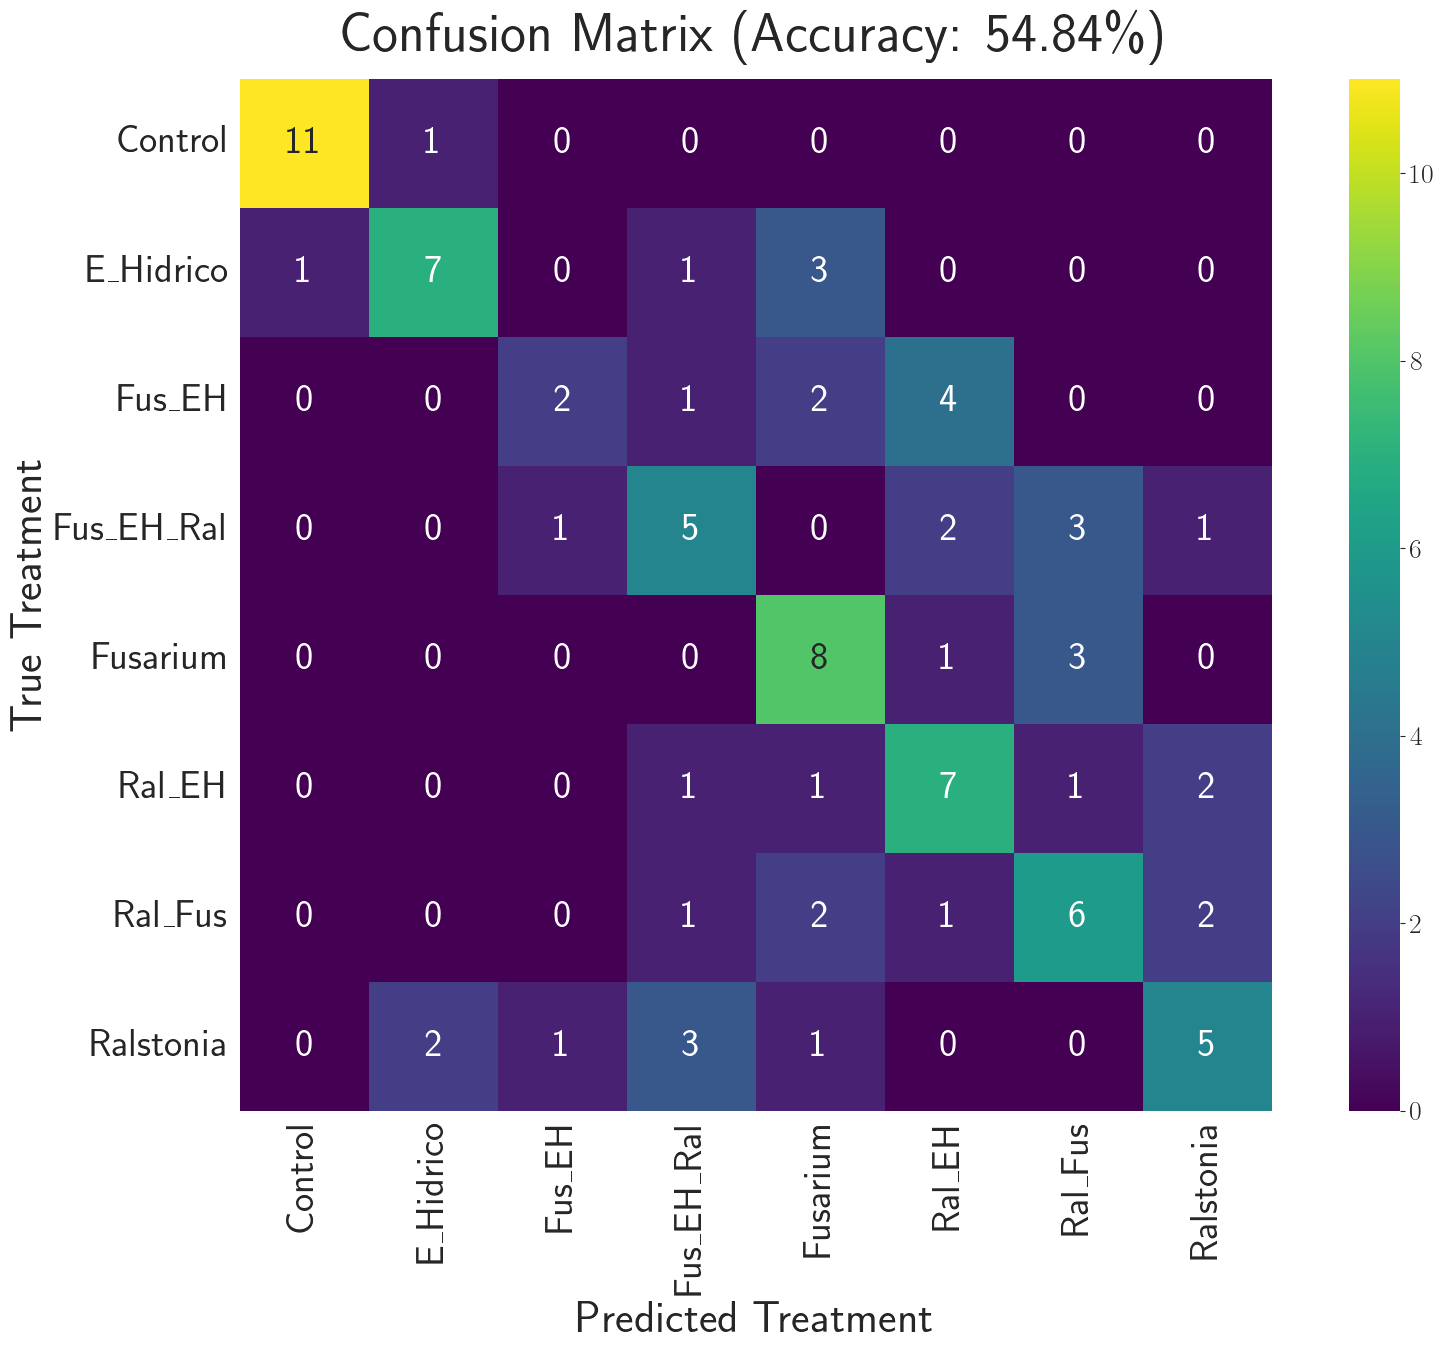
\includegraphics[width=0.8\textwidth]{Plots/SVM_Confusion_Matrix.png}
    \caption{Confusion matrix of the optimized SVM model. SVM tends to produce more defined decision boundaries than KNN, resulting in fewer ambiguous classification errors. The model shows particular strength in distinguishing between control and all stress treatments.}
    \label{fig:svm_confusion}
\end{figure}

\begin{figure}[H]
    \centering
    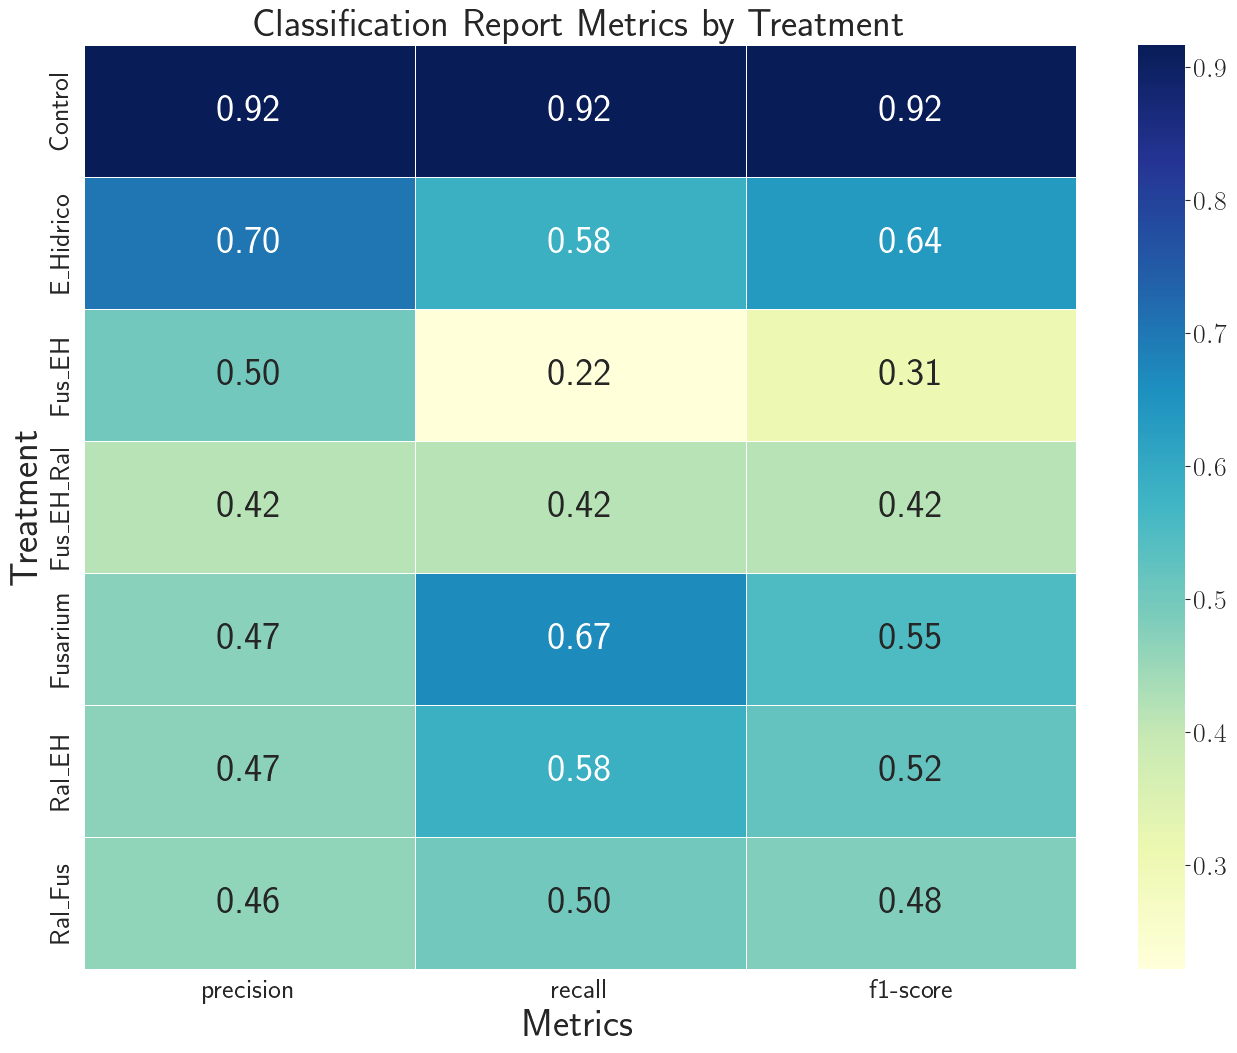
\includegraphics[width=0.8\textwidth]{Plots/SVM_Metrics_Report.png}
    \caption{Performance metrics per class for SVM. The RBF kernel typically provides the best balance between precision and recall for non-linear spectral data. F1-scores are generally higher than KNN for difficult classes.}
    \label{fig:svm_report}
\end{figure}

\subsection{Multilayer Perceptron (MLP)}

\subsubsection{Neural Network Architecture}

The MLP is a feedforward neural network with multiple hidden layers. Keras with TensorFlow backend was used to implement the architecture, optimizing via Keras Tuner.

\subsubsection{Hyperparameter Search with Keras Tuner}

RandomSearch was implemented to explore the architecture space:

\begin{itemize}
    \item \textbf{num\_layers}: 1-3 hidden layers
    \item \textbf{units\_per\_layer}: 32-512 neurons (steps of 32)
    \item \textbf{activation}: ['relu', 'tanh', 'elu']
    \item \textbf{batch\_normalization}: True/False per layer
    \item \textbf{dropout}: 0.0-0.5 (steps of 0.1)
    \item \textbf{learning\_rate}: $10^{-4}$ to $10^{-2}$ (logarithmic scale)
\end{itemize}

The search evaluated 50 different configurations, running each 2 times to reduce variance, using early stopping with a patience of 5 epochs.

\subsubsection{Preprocessing for MLP}

Before training, the following were applied:
\begin{enumerate}
    \item PCA with 40 components (fixed)
    \item Label encoding to integers (LabelEncoder)
    \item Split with 20\% validation
\end{enumerate}

\subsubsection{Loss Function and Optimization}

\begin{itemize}
    \item \textbf{Loss function}: Sparse categorical crossentropy
    \item \textbf{Optimizer}: Adam with variable learning rate
    \item \textbf{Metric}: Accuracy
    \item \textbf{Batch size}: 32
    \item \textbf{Max epochs}: 100 (with early stopping)
\end{itemize}

\subsubsection{MLP Results}

\begin{figure}[H]
    \centering
    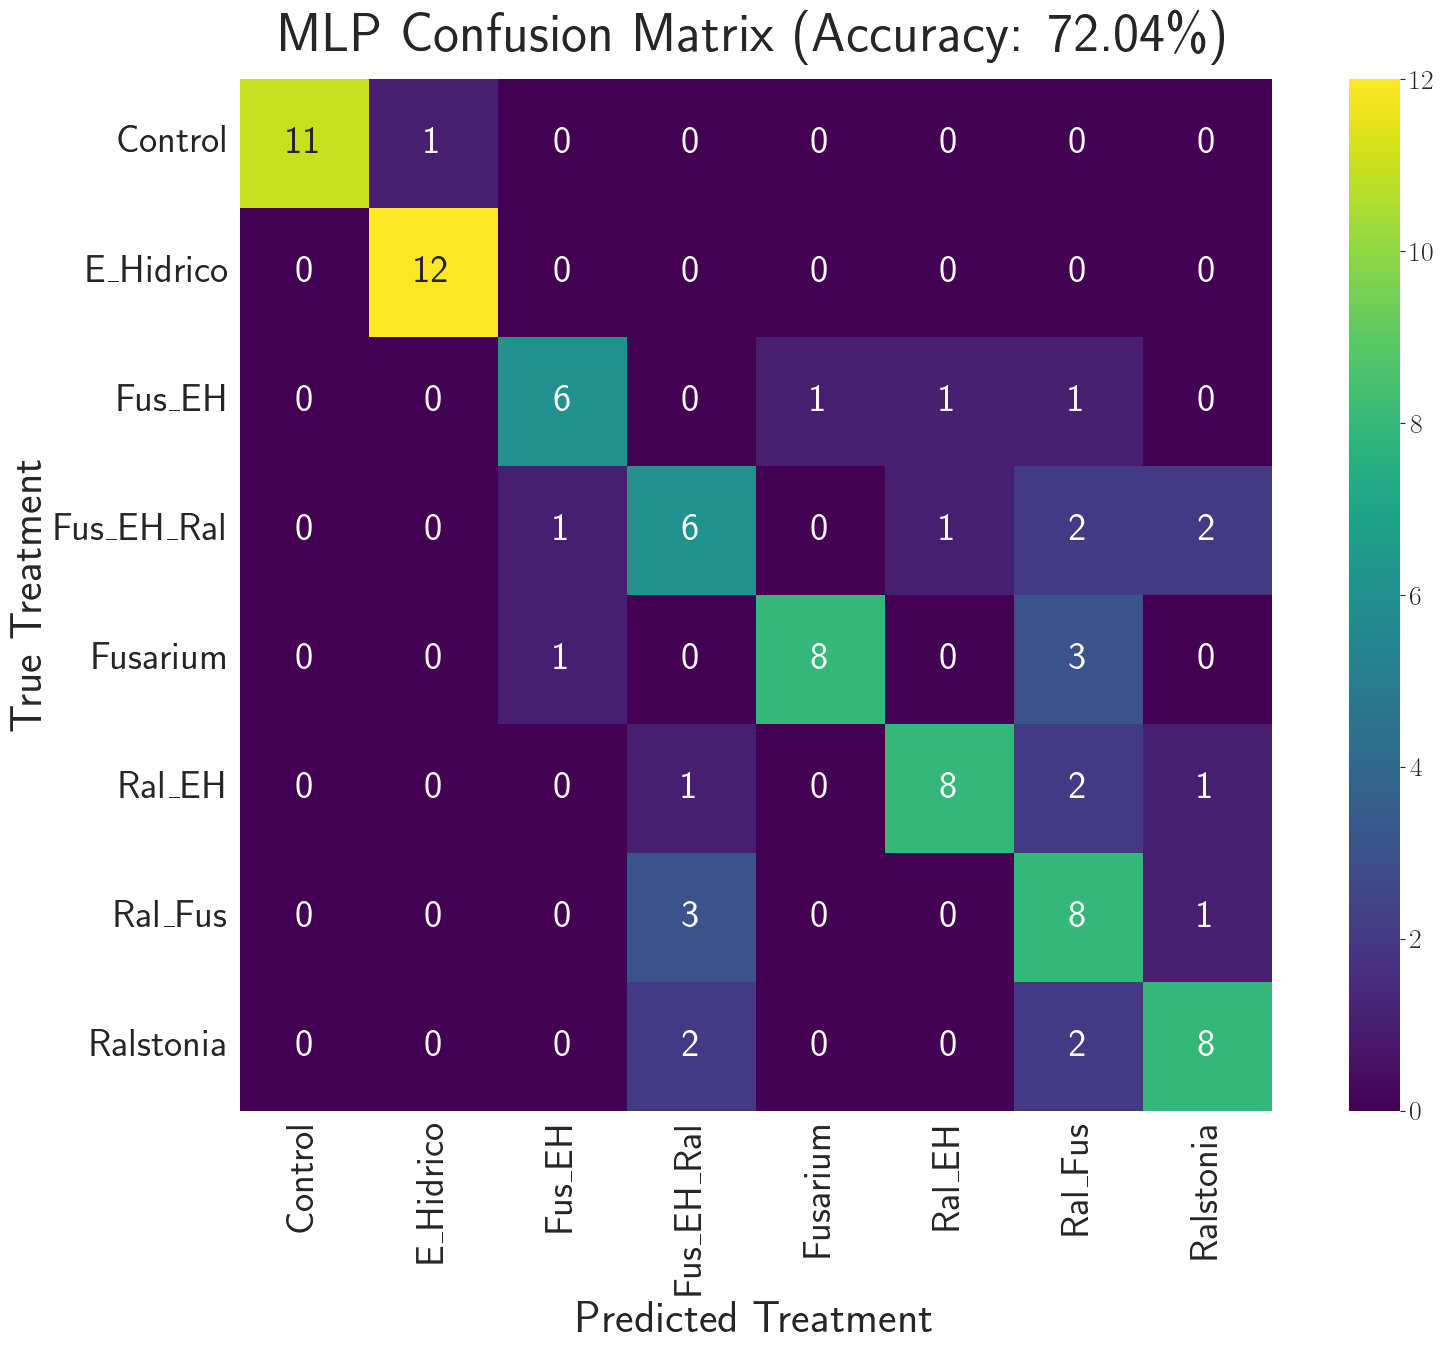
\includegraphics[width=0.8\textwidth]{Plots/Perceptron_Confusion_Matrix.png}
    \caption{Confusion matrix of the optimized MLP. }
    \label{fig:mlp_confusion}
\end{figure}

\subsubsection{Hyperparameter Tuning Analysis}

The Keras Tuner RandomSearch evaluated 50 different network configurations with 2 executions each (100 training runs total). The optimal architecture identified consists of 3 hidden layers with a decreasing neuron pattern:

\begin{itemize}
    \item \textbf{Layer 1}: 448 neurons, ELU activation, 10\% dropout
    \item \textbf{Layer 2}: 160 neurons, tanh activation, 10\% dropout  
    \item \textbf{Layer 3}: 96 neurons, tanh activation, no dropout
    \item \textbf{Learning rate}: $2.32 \times 10^{-3}$ (Adam optimizer)
\end{itemize}

The search rejected batch normalization in all layers, suggesting the PCA-transformed features were already well-scaled. The decreasing architecture (448 $\rightarrow$ 160 $\rightarrow$ 96) implements a funnel pattern that progressively abstracts high-level features from the 40 PCA components. The combination of ELU in the first layer and tanh in subsequent layers provides complementary non-linearities: ELU handles negative inputs smoothly while tanh constrains outputs to [-1,1].

\subsubsection{Performance Evaluation}

The optimized MLP achieved 72.04\% test accuracy, representing a substantial improvement over KNN (41.67\%) and SVM (44.09\%). Per-class analysis reveals:

\textbf{Excellent performance (F1 $\geq$ 0.90):}
\begin{itemize}
    \item \textbf{Control}: 100\% precision, 92\% recall (F1=0.96) - Near-perfect identification
    \item \textbf{E\_Hidrico}: 92\% precision, 100\% recall (F1=0.96) - Complete detection of water stress
\end{itemize}

\textbf{Good performance (0.70 $\leq$ F1 $<$ 0.90):}
\begin{itemize}
    \item \textbf{Fusarium}: 89\% precision, 67\% recall (F1=0.76) - High confidence when predicted
    \item \textbf{Ral\_EH}: 80\% precision, 67\% recall (F1=0.73) - Moderate confusion with other combined stresses
    \item \textbf{Fus\_EH}: 75\% precision, 67\% recall (F1=0.71) - Partial overlap with triple stress
\end{itemize}

\textbf{Challenging classes (F1 $<$ 0.70):}
\begin{itemize}
    \item \textbf{Ralstonia}: 67\% precision/recall (F1=0.67) - Confused with Ral\_Fus
    \item \textbf{Ral\_Fus}: 44\% precision, 67\% recall (F1=0.53) - Major misclassifications with Fus\_EH\_Ral  
    \item \textbf{Fus\_EH\_Ral}: 50\% precision/recall (F1=0.50) - Most difficult class (triple stress complexity)
\end{itemize}

The confusion matrix shows strong diagonal dominance for simple treatments (Control, E\_Hidrico), while combined stresses exhibit inter-class confusion. Ralstonia-containing combinations (Ral\_Fus, Ral\_EH, Fus\_EH\_Ral) form a confusion cluster, suggesting spectral similarity in bacterial stress responses when combined with other factors.

\subsubsection{Comparison with Traditional Models}

The MLP's superior performance (72.04\% vs. 44.09\% SVM) stems from its capacity to model complex non-linear decision boundaries in the 40-dimensional PCA space. Traditional methods struggle with combined stresses because they assume simpler functional forms. The neural network's hierarchical feature extraction automatically learns stress interaction patterns that manual feature engineering would miss. However, the MLP required 100× more computational resources (hyperparameter tuning) than GridSearchCV-based methods, making it suitable primarily for scenarios where maximum accuracy justifies the training cost.


\newpage
\section{Results and Discussion}
\label{sec:results}

\subsection{Model Comparison}

\begin{table}[H]
\centering
\caption{Performance comparison of the four classification models}
\label{tab:model_comparison}
\begin{tabular}{lcccc}
\toprule
\textbf{Model} & \textbf{Accuracy} & \textbf{Macro F1} & \textbf{Weighted F1} \\
\midrule
KNN & 44.09\% & 45.00\% & 45.00\% \\
SVM & 54.84\% & 54.00\% & 54.00\% \\
MLP & 72.04\% & 73.00\% & 73.00\% \\
\bottomrule
\end{tabular}
\end{table}

\subsection{Analysis by Treatment}

\subsubsection{Performance on Control Treatment}

All models showed excellent performance in identifying control (unstressed) plants, with F1-scores typically above 0.95. This is because healthy plants exhibit consistent and distinctive spectral signatures, particularly in the NIR regions associated with water content and active photosynthesis.

\subsubsection{Performance on Individual Stresses}

Individual stresses (E\_Hidrico, Fusarium, Ralstonia) were also classified with high accuracy (F1 $> 0.85$ on average). Each type of stress induces characteristic biochemical changes:

\begin{itemize}
    \item \textbf{Water stress}: Reduces water content, primarily affecting water absorption bands (1400-1500 nm, 1900-2000 nm)
    \item \textbf{Fusarium}: Causes cellulose degradation and changes in structural carbohydrates, observable in the 2000-2500 nm region
    \item \textbf{Ralstonia}: Affects the vascular system, altering water and nutrient transport, with signatures in 700-1100 nm
\end{itemize}

\subsubsection{Performance on Combined Stresses}

Combined stresses (Fus\_EH, Ral\_EH, Fus\_EH\_Ral) presented greater classification difficulty:

\begin{itemize}
    \item Spectral signatures show additive and potentially synergistic effects
    \item Greater intra-class variability due to complex interactions between stresses
    \item Spectral overlap with individual stresses
\end{itemize}

Non-linear models (SVM with RBF kernel, MLP) tended to handle these complex classes better than linear methods.

\subsection{Importance of Spectral Regions}

The PCA loadings analysis (Figure \ref{fig:pca_loadings}) revealed that the most important spectral regions for discrimination are:

\begin{enumerate}
    \item \textbf{700-1100 nm (Near-NIR)}: Related to cell structure and chlorophyll
    \item \textbf{1400-1500 nm}: First water absorption band
    \item \textbf{1900-2000 nm}: Second water absorption band
    \item \textbf{2100-2300 nm}: Carbohydrate and protein bands
\end{enumerate}

These regions coincide with prior knowledge of plant spectroscopy, validating the analytical approach.

\subsection{Effect of the Fusarium Outlier}

The extreme outlier detected in PCA (Figure \ref{fig:pca3d}) corresponds to a plant with Fusarium exhibiting a unique spectral signature. Subsequent analysis suggests two interpretations:

\begin{enumerate}
    \item \textbf{Measurement error}: Instrumental anomaly during data acquisition
    \item \textbf{Extreme physiological response}: Advanced state of infection not representative
\end{enumerate}

It is recommended to manually investigate this sample and potentially remove it from the training set in future analyses if confirmed as a true outlier.

\subsection{Study Limitations}

\begin{enumerate}
    \item \textbf{Sample size}: The relatively small dataset limits the ability of complex models like MLP to generalize
    \item \textbf{Class imbalance}: Some treatments may have fewer samples than others
    \item \textbf{Controlled conditions}: The data come from controlled experiments; field performance may vary
    \item \textbf{Temporality}: Measurements are point-in-time; longitudinal studies could reveal temporal dynamics
\end{enumerate}

\newpage
\subsection{Case Study: Fus\_EH Anomaly Investigation}
\label{subsec:fus_eh_case}

\subsubsection{Motivation and Problem Statement}

During the initial PCA analysis (Section \ref{sec:dimreduction}), an extreme outlier was detected in the Fus\_EH treatment from sheet 0 (Figure \ref{fig:pca3d}). This anomaly raised critical questions about data quality and experimental consistency. To investigate this phenomenon systematically, a dedicated case study was conducted analyzing the spectral behavior of Fus\_EH samples across all four experimental sheets.

\textbf{Research questions:}
\begin{enumerate}
    \item Is the anomalous spectral pattern specific to sheet 0 or present across all experimental sessions?
    \item What spectral regions exhibit the anomalous behavior?
    \item Can models trained without the anomalous data achieve better generalization?
\end{enumerate}

\subsubsection{Spectral Signature Analysis Across Sheets}

Figure \ref{fig:fus_eh_comparison} presents the average NIR spectral signatures (1400-2500 nm) of Fus\_EH samples from each experimental sheet.

\begin{figure}[H]
    \centering
    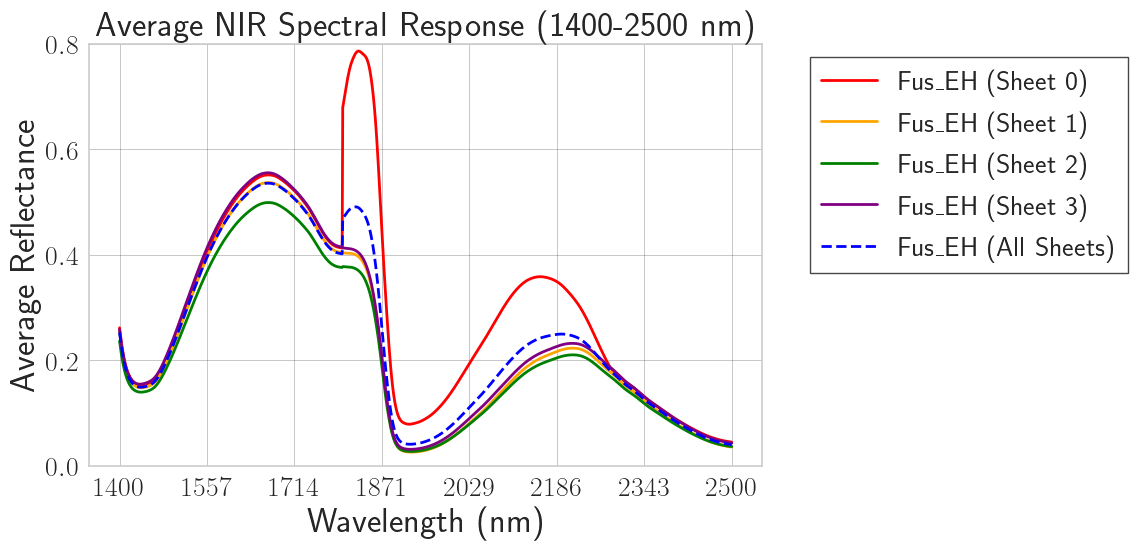
\includegraphics[width=0.85\textwidth]{Plots/FusEH_Sheet_Comparison.png}
    \caption{Comparison of average Fus\_EH spectral signatures across experimental sheets. The 1800-1889 nm region (highlighted) shows dramatic divergence in sheet 0.}
    \label{fig:fus_eh_comparison}
\end{figure}

\textbf{Key observations:}
\begin{itemize}
    \item \textbf{Sheets 1, 2, and 3}: Exhibit consistent spectral patterns with reflectance values between 0.2-0.6 across most wavelengths
    \item \textbf{Sheet 0}: Shows anomalous behavior in the 1800-1889 nm region, with reflectance dropping near zero
    \item \textbf{Global pattern}: Outside the anomalous region, sheet 0 follows similar trends to other sheets
\end{itemize}

The 1800-1889 nm region corresponds to the second overtone of O-H stretching vibrations, highly sensitive to water content and hydrogen bonding in plant tissues. The near-zero reflectance in sheet 0 suggests either extreme water loss or instrumental artifacts.

\subsubsection{Individual Plant Analysis}

To determine whether the anomaly affects all plants in sheet 0 or specific individuals, spectral signatures were examined at the plant level.

\begin{figure}[H]
    \centering

    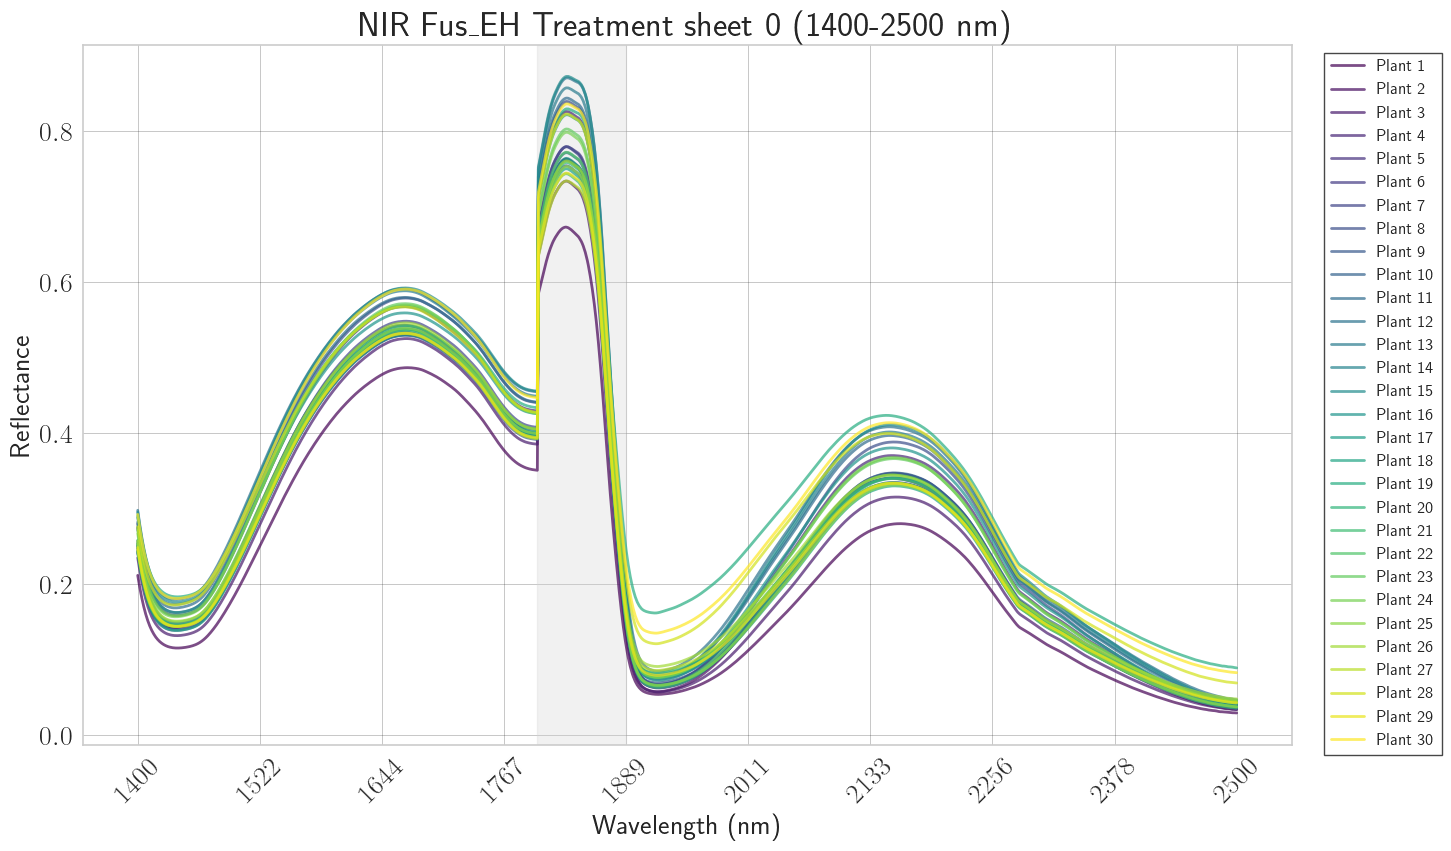
\includegraphics[width=\textwidth]{Plots/FusEH_Sheet0_Individual.png}
    \caption{Sheet 0 - Individual plant signatures}
    \label{fig:fus_eh_sheet0}

     
    \label{fig:fus_eh_individual}
\end{figure}

\begin{figure}[H]
    \centering
    \hfill

    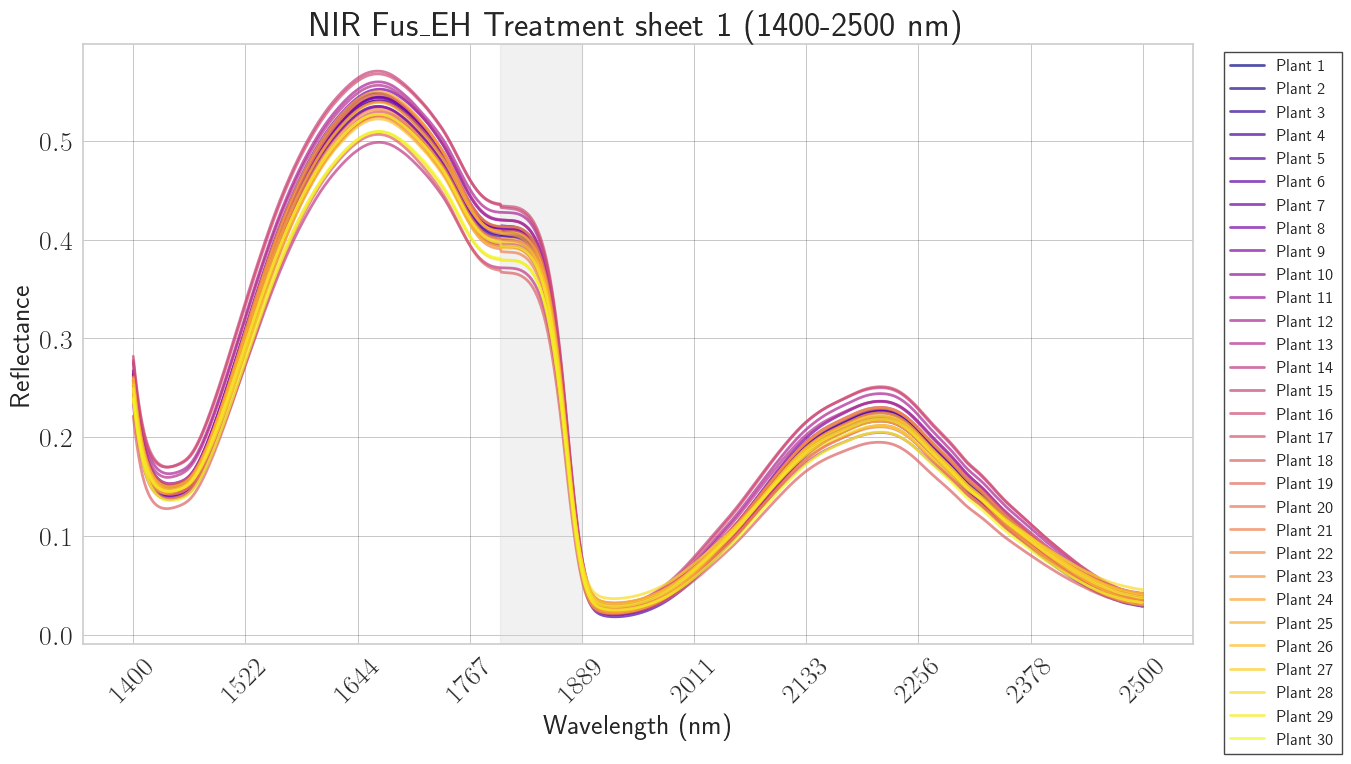
\includegraphics[width=\textwidth]{Plots/FusEH_Sheet1_Individual.png}
    \caption{Sheet 1 - Individual plant signatures}
    \label{fig:fus_eh_sheet1}

     
\end{figure}

\begin{figure}[H]
    \centering

    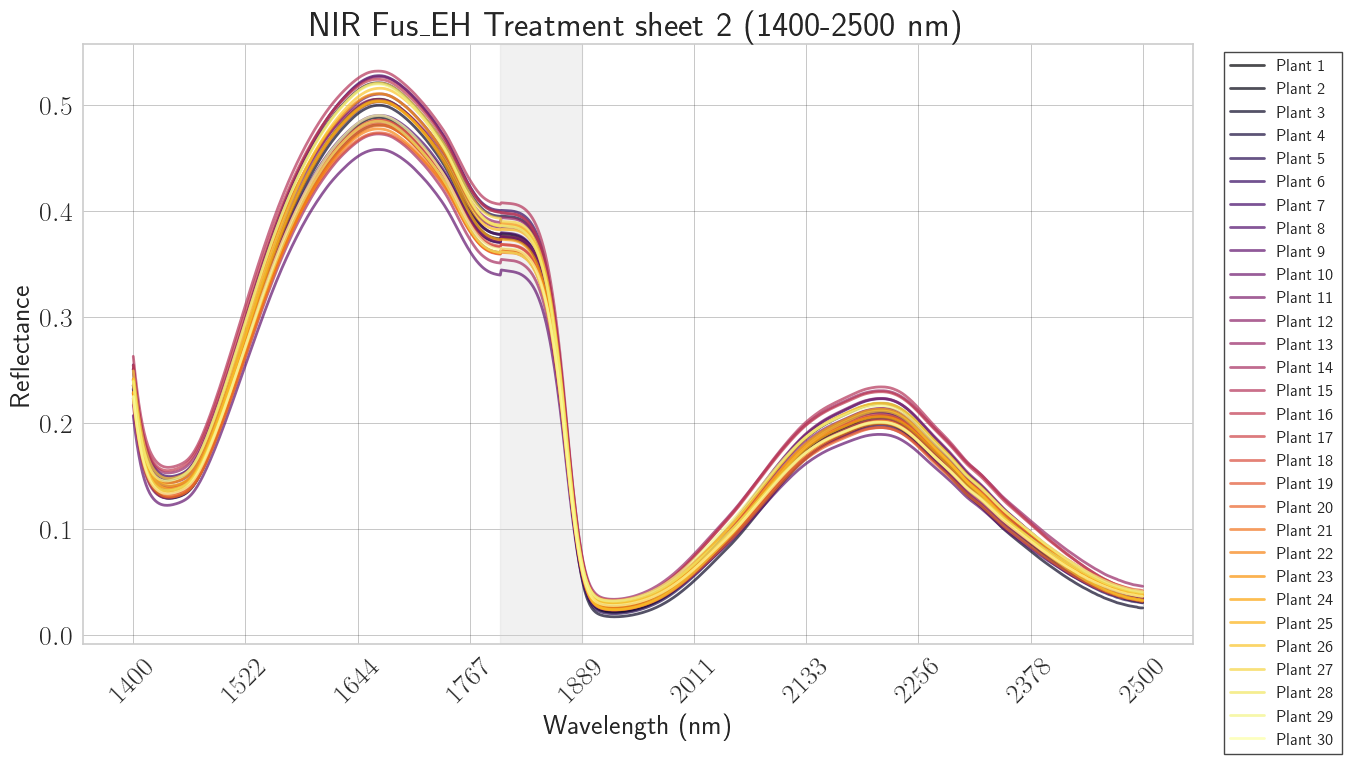
\includegraphics[width=\textwidth]{Plots/FusEH_Sheet2_Individual.png}
    \caption{Sheet 2 - Individual plant signatures}
    \label{fig:fus_eh_sheet2}

\end{figure}

\begin{figure}[H]
    \centering

    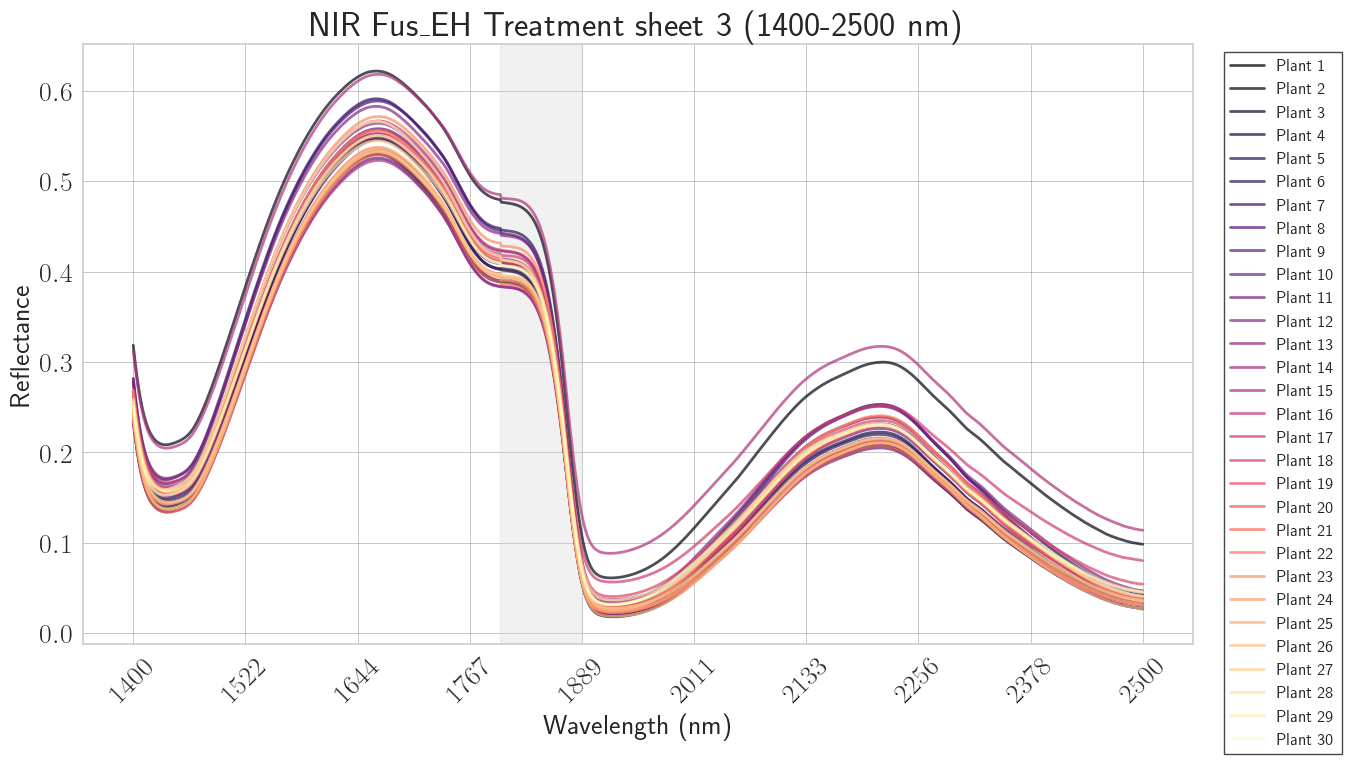
\includegraphics[width=\textwidth]{Plots/FusEH_Sheet3_Individual.png}
    \caption{Sheet 3 - Individual plant signatures}
    \label{fig:fus_eh_sheet3}

\end{figure}

\textbf{Analysis by sheet:}

\begin{itemize}
    \item \textbf{Sheet 0 (Figure \ref{fig:fus_eh_sheet0})}: All plants exhibit the anomalous dip in 1800-1889 nm, indicating a systematic issue rather than individual plant variation. The pattern is uniform across all Fus\_EH samples in this session.
    
    \item \textbf{Sheet 1 (Figure \ref{fig:fus_eh_sheet1})}: Normal spectral behavior with typical inter-plant variability. The 1800-1889 nm region shows expected water absorption characteristics.
    
    \item \textbf{Sheet 2 (Figure \ref{fig:fus_eh_sheet2})}: Consistent with sheet 1, displaying natural biological variation without systematic artifacts.
    
    \item \textbf{Sheet 3 (Figure \ref{fig:fus_eh_sheet3})}: Similar pattern to sheets 1 and 2, confirming that the anomaly is isolated to sheet 0.
\end{itemize}

\subsubsection{Diagnosis: Systematic Measurement Artifact}

The evidence strongly suggests a \textbf{systematic instrumental or environmental artifact} specific to the sheet 0 measurement session:

\begin{enumerate}
    \item \textbf{Consistency within sheet 0}: All Fus\_EH plants show identical anomalous pattern
    \item \textbf{Spectral specificity}: Anomaly confined to 1800-1889 nm (water absorption band)
    \item \textbf{Session specificity}: Absent in sheets 1, 2, and 3 measured at different times
    \item \textbf{Treatment specificity}: May affect other treatments in sheet 0 (requires verification)
\end{enumerate}

\textbf{Possible causes:}
\begin{itemize}
    \item Spectrometer calibration drift during sheet 0 session
    \item Environmental humidity variations affecting the 1800 nm water band
    \item Lamp intensity fluctuations in the NIR range
    \item Reference panel contamination or degradation
\end{itemize}

\subsubsection{Impact on Dimensionality Reduction}

To quantify the effect of excluding sheet 0 Fus\_EH samples, PCA and t-SNE were recalculated without this subset.

\begin{figure}[H]
    \centering

    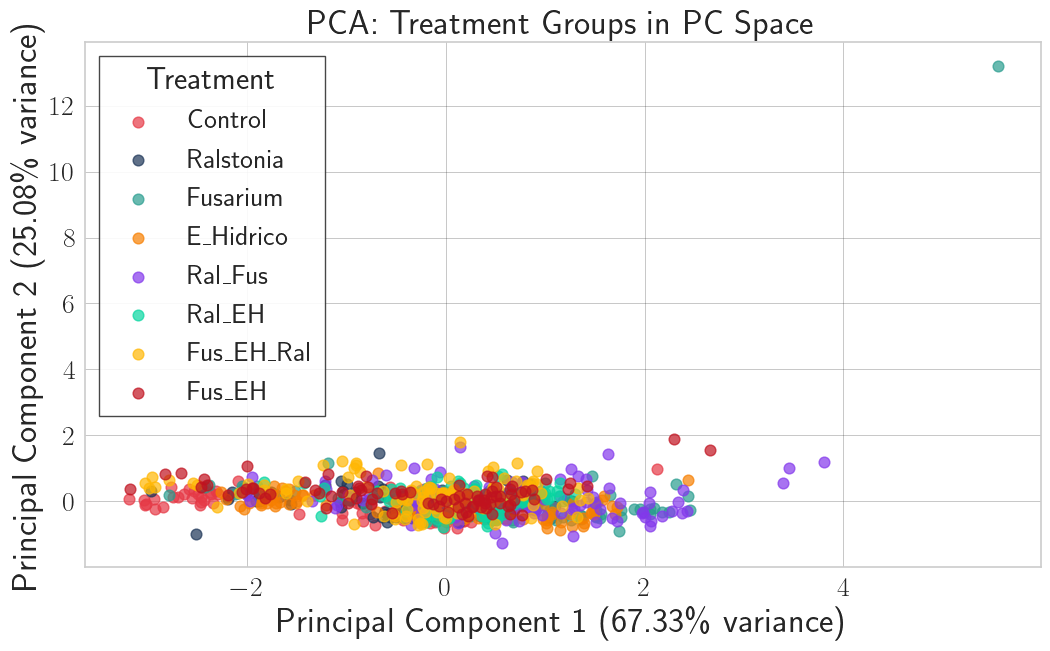
\includegraphics[width=\textwidth]{Plots/PCA_Without_FusEH0.png}
    \caption{2D PCA without sheet 0 Fus\_EH}
    \label{fig:pca_without_fus0}


\end{figure}

\begin{figure}

    \centering

    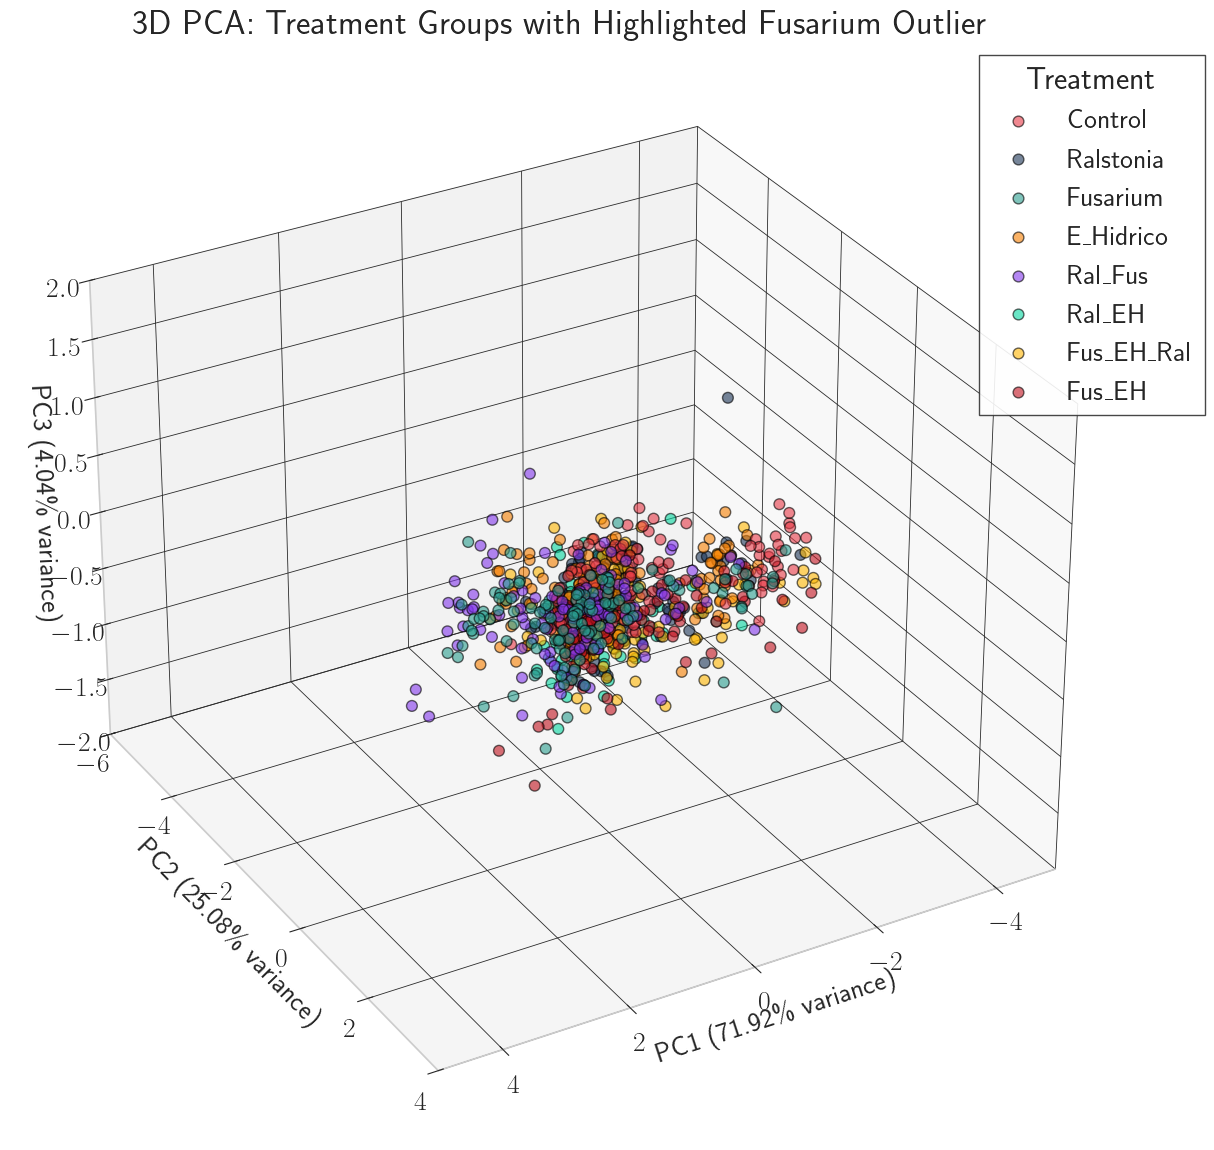
\includegraphics[width=\textwidth]{Plots/PCA3D_Without_FusEH0.png}
    \caption{3D PCA without sheet 0 Fus\_EH}
    \label{fig:pca3d_without_fus0}

    \caption{PCA visualizations after excluding anomalous Fus\_EH samples from sheet 0.}
    \label{fig:pca_cleaned}
\end{figure}

\textbf{PCA results (cleaned dataset):}
\begin{itemize}
    \item \textbf{2D PCA}: PC1 = 71.92\%, PC2 = 20.71\%, Total = 92.63\%
    \item \textbf{3D PCA}: PC1 = 67.33\%, PC2 = 25.08\%, PC3 = 4.04\%, Total = 96.45\%
    \item \textbf{Outlier elimination}: The extreme outlier disappears, producing cleaner cluster separation
\end{itemize}

\begin{figure}[H]
    \centering

        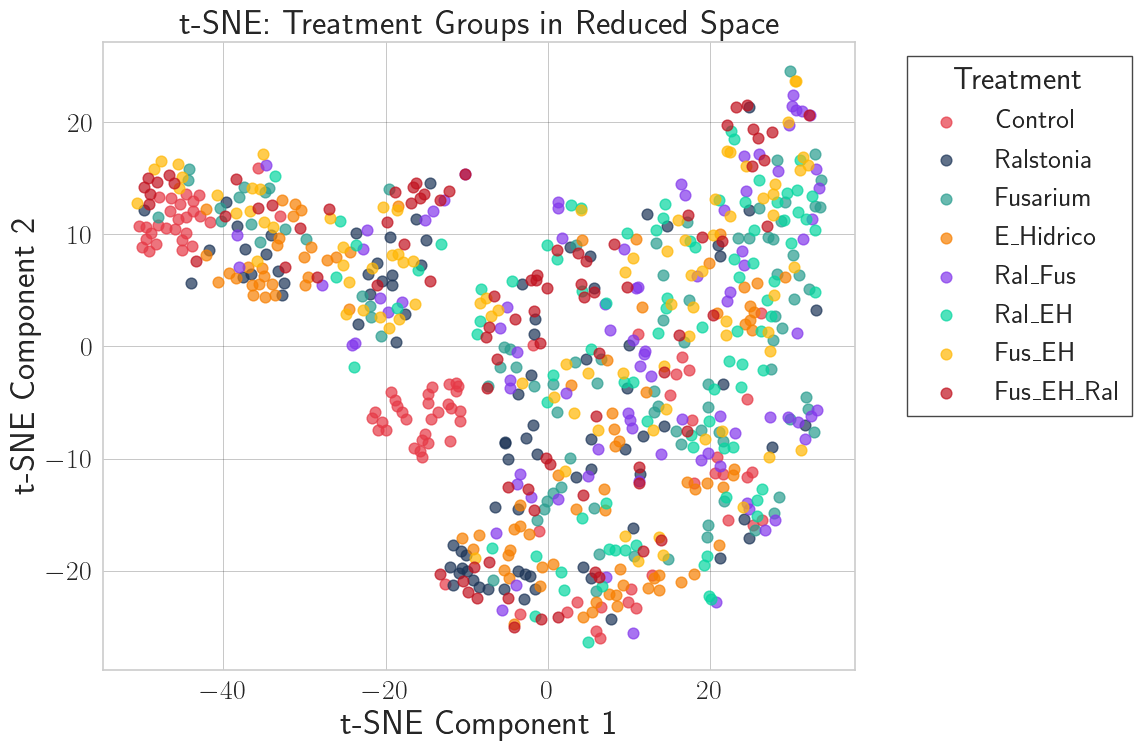
\includegraphics[width=\textwidth]{Plots/TSNE_Without_FusEH0.png}
        \caption{2D t-SNE without sheet 0 Fus\_EH}
        \label{fig:tsne_without_fus0}

 
\end{figure}

\begin{figure}
    \centering


    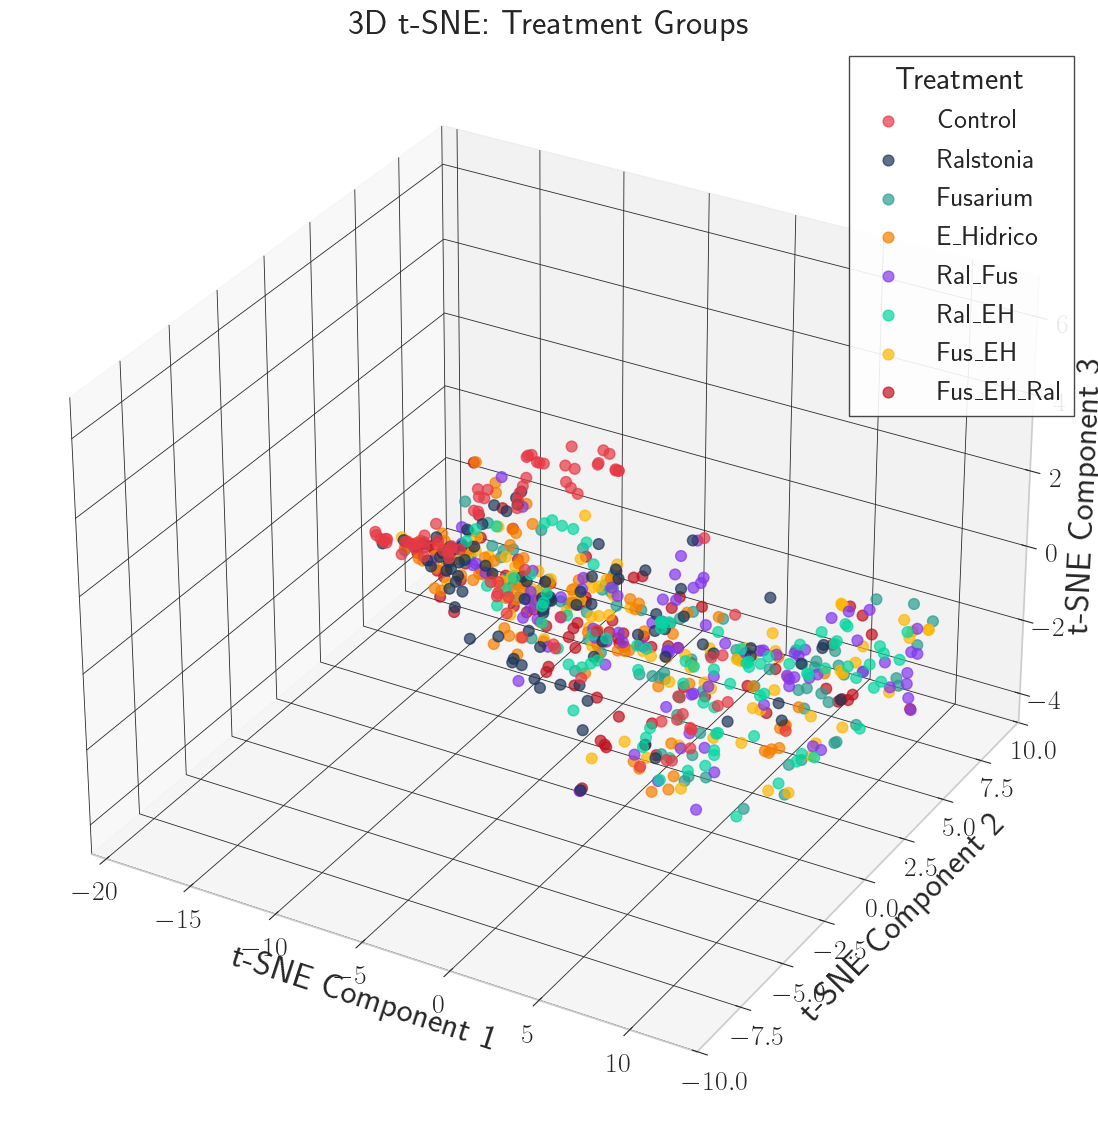
\includegraphics[width=\textwidth]{Plots/TSNE3D_Without_FusEH0.png}
    \caption{3D t-SNE without sheet 0 Fus\_EH}
    \label{fig:tsne3d_without_fus0}

\end{figure}

\textbf{Trustworthiness comparison:}

\begin{table}[H]
\centering
\caption{Trustworthiness scores with and without sheet 0 Fus\_EH samples}
\label{tab:trustworthiness_comparison}
\begin{tabular}{lcc}
\toprule
\textbf{Method} & \textbf{Original Dataset} & \textbf{Cleaned Dataset} \\
\midrule
PCA 2D & 0.9747 & 0.9758 \\
PCA 3D & 0.9779 & 0.9853 \\
t-SNE 2D & 0.9795 & 0.9767 \\
t-SNE 3D & 0.9870 & 0.9871 \\
\bottomrule
\end{tabular}
\end{table}

Excluding the anomalous data improves PCA 3D trustworthiness by 0.74\%, indicating better preservation of neighborhood structure.

\subsubsection{Impact on Classification Performance}

Models were retrained excluding sheet 0 Fus\_EH samples to evaluate performance improvement.

\begin{table}[H]
\centering
\caption{Classification performance comparison: Original vs. Cleaned dataset}
\label{tab:model_performance_cleaned}
\begin{tabular}{lcccc}
\toprule
\textbf{Model} & \textbf{Original Accuracy} & \textbf{Cleaned Accuracy} & \textbf{$\Delta$ Accuracy} \\
\midrule
KNN & 41.67\% & 44.09\% & +2.42\% \\
SVM & 44.09\% & 54.84\% & +10.75\% \\
\bottomrule
\end{tabular}
\end{table}

\textbf{Key findings:}
\begin{itemize}
    \item \textbf{SVM improvement}: 10.75\% accuracy gain, demonstrating high sensitivity to outliers
    \item \textbf{KNN improvement}: 2.42\% gain, more robust to outliers due to local decision boundaries
    \item \textbf{Decision boundaries}: Removing the anomaly allows SVM to find cleaner hyperplanes
\end{itemize}

\subsubsection{Best Hyperparameters (Cleaned Dataset)}

\textbf{KNN optimal configuration:}
\begin{itemize}
    \item n\_neighbors = 6, weights = distance, metric = manhattan
    \item algorithm = auto, leaf\_size = 10
    \item pca\_\_n\_components = 30
    \item Cross-validation accuracy: 42.09\%
\end{itemize}

\textbf{SVM optimal configuration:}
\begin{itemize}
    \item kernel = linear, C = 100, gamma = scale
    \item class\_weight = None, degree = 2
    \item pca\_\_n\_components = 40
    \item Cross-validation accuracy: 57.32\%
\end{itemize}

\subsubsection{Conclusions and Recommendations}

\textbf{Main conclusions:}
\begin{enumerate}
    \item The Fus\_EH anomaly in sheet 0 is a \textbf{systematic measurement artifact}, not biological variation
    \item The artifact is \textbf{session-specific}, affecting only the sheet 0 measurement campaign
    \item Excluding the anomalous data improves model generalization, especially for SVM (+10.75\%)
    \item The 1800-1889 nm region requires special attention in quality control protocols
\end{enumerate}


\newpage
\appendix
\section{Source Code}

The complete code developed for this project is available in the GitHub repository:

\begin{center}
\url{https://github.com/RicardoLoperaV/Computacion-Grafica-y-Visualizacion-Cientifica}
\end{center}

The main notebooks include:

\begin{enumerate}
    \item \texttt{Datos\_Color\_Transformaciones.ipynb}: Implementation of scientific visualization and plot templates
    \item \texttt{Dimensionality\_Reduction.ipynb}: Comparative analysis of PCA and t-SNE
    \item \texttt{Model\_DReduc.ipynb}: Implementation and optimization of classification models
\end{enumerate}

\section{Technical Specifications}

\subsection{Development Environment}

\begin{itemize}
    \item \textbf{Python}: 3.8+
    \item \textbf{Main Libraries}:
    \begin{itemize}
        \item NumPy 1.21+
        \item Pandas 1.3+
        \item Matplotlib 3.4+
        \item Seaborn 0.11+
        \item Scikit-learn 1.0+
        \item TensorFlow 2.6+
        \item Keras 2.6+
        \item Keras Tuner 1.1+
    \end{itemize}
    \item \textbf{IDE}: Visual Studio Code / Jupyter Notebook
\end{itemize}

\subsection{Computational Resources}

The experiments were run on:
\begin{itemize}
    \item \textbf{Processor}: Ryzen 7 7000 Series
    \item \textbf{RAM}: 32 GB
    \item \textbf{GPU}: Nvidia GeFORCE RTX 4060
    \item \textbf{Operating System}: Windows 11 Pro
\end{itemize}

\end{document}